% ===========================================================================
% NeuroPLC —— 从PyTorch到PLC：面向IEC 61131-3控制器的
%           智能故障诊断自动化代码生成与结构可验证编译
% ===========================================================================

\documentclass[journal,onecolumn]{IEEEtran}

% ── 中文支持 ──
\usepackage[UTF8]{ctex}
\setCJKmainfont{SimSun}[BoldFont=SimHei,ItalicFont=KaiTi]
\setCJKsansfont{SimHei}
\setCJKmonofont{FangSong}

% ── Packages ──
\usepackage{amsmath,amssymb,amsfonts,amsthm}
\usepackage{graphicx}
\usepackage{booktabs}
\usepackage{multirow}
\usepackage{array}
\usepackage{tabularx}
\usepackage{makecell}
\usepackage{algorithm}
\usepackage{algpseudocode}
\usepackage[colorlinks=true,linkcolor=blue,citecolor=blue,urlcolor=blue]{hyperref}
\usepackage[capitalise,noabbrev]{cleveref}
\usepackage{cite}
\usepackage{xcolor}
\usepackage{pifont}
\usepackage{xspace}
\usepackage{enumitem}

% ── IEEEtran 双栏浮空控制 ──
\usepackage{dblfloatfix}

% ── 编译器指称语义括号 ──
\newcommand{\llbracket}{[\![}
\newcommand{\rrbracket}{]\!]}

% ── 宏定义 ──
\newcommand{\neuroplc}{NeuroPLC\xspace}
\newcommand{\kan}{KAN\xspace}
\newcommand{\scl}{SCL\xspace}
\newcommand{\plc}{PLC\xspace}

% ── 分类标记 ──
\newcommand{\cmark}{\ding{51}}
\newcommand{\xmark}{\ding{55}}

% ── 数学算子 ──
\DeclareMathOperator*{\argmax}{arg\,max}
\DeclareMathOperator*{\argmin}{arg\,min}

% ── 定理环境（中文 + amsthm 风格统一） ──
\theoremstyle{definition}
\newtheorem{definition}{定义}
\theoremstyle{plain}
\newtheorem{theorem}{定理}
\newtheorem{proposition}{命题}
\newtheorem{lemma}{引理}
\newtheorem{corollary}{推论}
\theoremstyle{remark}
\newtheorem{remark}{注记}
\newtheorem{conjecture}{猜想}

% ── 全局表格样式 ──
\renewcommand{\tabcolsep}{4pt}
\renewcommand{\arraystretch}{1.15}

% ── 全局列表间距 ──
\setlist{nosep,leftmargin=*}

% ── cleveref 中文标签 ──
\crefname{theorem}{定理}{定理}
\crefname{proposition}{命题}{命题}
\crefname{lemma}{引理}{引理}
\crefname{definition}{定义}{定义}
\crefname{remark}{注记}{注记}
\crefname{figure}{图}{图}
\crefname{table}{表}{表}
\crefname{equation}{式}{式}
\crefname{section}{节}{节}
\crefname{algorithm}{算法}{算法}

\begin{document}

% ===========================================================================
% 标题
% ===========================================================================
\title{NeuroPLC：从PyTorch到IEC 61131-3 SCL的结构可验证编译\\ 及其在工业PLC上的应用}

\author{刘甫悦，\IEEEmembership{桂林电子科技大学，广西桂林 541004}}

\markboth{IEEE TRANSACTIONS ON INDUSTRIAL INFORMATICS, VOL. XX, NO. XX, 2026}%
         {Liu: NeuroPLC --- Structurally Verifiable Compilation from PyTorch to SCL}

\maketitle

% ── 排版控制 ──
\clubpenalty=10000
\widowpenalty=10000
\raggedbottom
\emergencystretch=1em

% ===========================================================================
% 摘要
% ===========================================================================
\begin{abstract}
编译器能否证明部署到PLC上的神经网络代码忠实地保留了训练模型的行为？本文证明，答案不取决于编译器工程，而取决于模型的\textbf{架构}。我们提出了\textbf{结构可验证神经网络（Structurally Verifiable Neural Network, SVNN）}框架：两个条件——操作类型封闭性和单变量有界性——足以让编译器仅凭模型参数计算出对所有输入有效的有限逐输出误差界（定理2）。标准MLP可证明不满足这些条件（命题1）；采用B样条激活函数的Kolmogorov-Arnold网络（KAN）则满足。违反条件使紧致界计算成为NP难问题（定理5）；满足更强的收缩条件则产生随深度\textit{改善}的泛化界$\Delta L \leq O(\gamma^L/\sqrt{n})$（定理6）。SVNN框架由此定义了一条\textbf{可编译前沿}——一条原则性的边界，将部署行为可在设计时认证的架构与需要运行时测试的架构分隔开来。

我们通过\neuroplc{}实例化SVNN——这是首个将PyTorch模型翻译为西门子S7-1200/1500 IEC~61131-3 SCL的基于IR的编译器。三种验证机制组合为端到端保证：(i)~一次性Z3 SMT证明，确认4/6种IR操作类型模板对所有可能参数均正确；(ii)~512个逐函数Z3证明组装为机器可检查的端到端证书，由约200行可信检查器验证；(iii)~符号结构仿射算术，比区间算术紧致$2.2\times$（与$\sqrt{d}$随机权重基线相比达$3.1\times$，安全因子$8.5\times$）。KAN的分解是\textit{结构必然性}：同规模KAN与MLP分别获得512/512与0/16的Z3可验证组件。该框架扩展到ChebyKAN（切比雪夫多项式基，命题2，496/512 Z3可验证）。三层KAN实现608/608 Z3验证（100\%），NeuroPLC的DA界比CROWN-IBP紧致$85\times$，生成的SCL在TIA Portal V21中以\textbf{0错误、0警告}编译（45.2~KB，S7-1200预算的90.4\%）。在CWRU（99.93\%）、XJTU-SY全寿命试验（91.7\%微调，512/512 Z3保留）和MNIST（98.6\%）上验证。
\end{abstract}

\begin{IEEEkeywords}
Kolmogorov-Arnold网络，IEC 61131-3，结构化文本（SCL），神经网络编译器，结构可验证性，仿射算术，SMT验证，组合认证，切比雪夫多项式网络，泛化界。
\end{IEEEkeywords}

% ===========================================================================
% 一、引言
% ===========================================================================
\section{引言}
\label{sec:intro}

一个在CWRU数据集上达到99.93\%故障诊断准确率的神经网络——孤立地看——无法部署到控制其监测设备的PLC上。其原因不是偶发的，而是结构性的：PLC以确定性扫描周期执行IEC~61131-3结构化控制语言（SCL），而非PyTorch；其工作内存预算（西门子S7-1200 CPU~1211C仅50~KB）排除了ML推理框架所需的运行时库；而——本文要解决的问题——没有任何现有工具能够\textit{认证}编译后的神经网络在工业控制器的定点REAL算术中保留其训练行为。现有ML$\to$PLC工具（RTNNIgen~\cite{rtnnigen2024}、MLconverter~\cite{mlconverter2025}、ICSML~\cite{icsml2023}）仅提供经验测试集验证；唯一的KAN-on-PLC先例（Corr\^ea~\cite{correa2024kanplc}，USP 2024）依赖通过Snap7的分布式PC-to-PLC通信，而非本地SCL编译，且未提供任何正确性保证。通用编译器（TVM、ONNX Runtime）无法以IEC~61131-3为目标。四条独立研究路线汇聚于同一观察——KAN的单变量B样条结构本质上适合基于LUT的硬件评估——涵盖FPGA（KANEL\'{E}~\cite{kanele2026}，ISFPGA~2026最佳论文）、MCU（LUT-KAN~\cite{lutkan2025}）、TinyML（KAN-SoC~\cite{kan_soc_2025}）和形式化验证（Schwartz等~\cite{schwartz2026optimal}）。然而，\textit{无一}提供具有设计时认证的端到端PyTorch-to-IEC~61131-3编译器——这正是本文交付的组合。

本文的\textit{结构洞察}是：认证差距不是编译器工程问题——而是一个\textit{架构}问题。编译器能否计算设计时正确性保证，取决于网络架构是否分解为误差传播封闭的操作。我们通过\textbf{SVNN}框架（{\S}\ref{sec:svnn}）形式化了这一洞察：两个结构条件（操作类型封闭性、单变量有界性）足以让编译器为验证域内所有输入计算有限、参数可计算的逐输出误差界（定理2）。KAN满足这些条件；采用SiLU/Sigmoid/Tanh激活的标准MLP可证明不满足（命题1）。SVNN由此定义了一条\textbf{可编译前沿}：将部署行为可在设计时认证的架构与需要运行时测试的架构分隔的原则性边界。

我们在\neuroplc{}中实现了这一框架——这是首个将PyTorch KAN翻译为西门子S7-1200/1500 SCL的基于IR的编译器。编译器是SVNN的\textit{概念验证}——而非其主要贡献。三种验证机制建立保证：（1）Z3 SMT编译器模板验证（一次性，4/6种IR操作类型证明）；（2）组合证书（512个逐函数证明$\to$约200行端到端可信检查器）；（3）符号结构仿射算术（比区间算术紧致$2.2\times$，与$\sqrt{d}$随机权重基线相比达$3.1\times$）。KAN的B样条分解是\textit{结构必然性}：同规模MLP $[28,16,4]$仅0/16 Z3可验证组件，而KAN为512/512。

Liu等~\cite{liu2024kan}提出的KAN将固定激活函数（ReLU）替换为置于网络边上的可学习B样条函数——这一结构差异是可验证性的关键。B样条激活本质上是分段多项式，使得确定性查表（LUT）编译成为可能，且具有保证的误差界（$\varepsilon \leq M_2\Delta^2/8$）。每条B样条边仅需68字节LUT存储即可编译~\cite{lutkan2025}，在资源受限硬件上实现7--25$\times$推理加速。

先前ML$\to$PLC工具确立了编译是\textit{可能的}，但未解决是否可以\textit{认证}的问题。RTNNIgen~\cite{rtnnigen2024}将Keras模型转换为IEC~61131-3结构化文本；MLconverter~\cite{mlconverter2025}以scikit-learn为ABB控制器目标。两者仅提供经验测试集验证——一种从ML基准测试继承的正确性模型，对安全关键PLC部署不足。这些工具留下的差距不是实现差距（"它们不够努力"）——而是\textit{架构}差距。我们的核心发现是：对于违反SVNN条件的架构，任何编译器工程都无法弥合这一差距（定理5）。SVNN框架解释了\textit{为何}先前工具未提供保证——它们的目标架构在结构上排除了这种可能。NeuroPLC是首个将训练后的PyTorch模型编译为IEC~61131-3 SCL\textit{并}为这种编译何时可以认证提供形式化体系的编译器。

\textbf{范围。}\neuroplc{}将分类器（KAN/MLP）编译为SCL。频域特征假设通过DSP预提取并通过PROFINET/OPC UA传输。PLC端的时域子集也可编译（E51）。本文贡献：

\begin{enumerate}
    \item \textbf{理论（结构可验证性）：}提出\textbf{SVNN}框架（{\S}\ref{sec:svnn}），形式化神经网络编译器能够提供设计时正确性保证的架构条件。两个充分条件（操作类型封闭性、单变量有界性）保证任意有限深度网络的有限、参数可计算的先验误差界；第三个收缩性精炼将其锐化为与深度无关的界（\textbf{定理2}）。\textbf{命题1}确立了标准MLP（ReLU、Sigmoid、Tanh）\textit{不}满足这些条件。该框架将编译器设计问题从"能否验证任意架构？"重构为"哪些架构本质可验证？"——这一转变的影响远超PLC领域。
    \item \textbf{系统（编译器）：}\neuroplc{}——首个PyTorch-to-西门子SCL编译器，使用与KAN的SVNN分解匹配的6操作IR（{\S}\ref{sec:ir}）。生成的SCL在TIA Portal V21中于S7-1200和S7-1500上以\textbf{0e 0w}编译（{\S}\ref{sec:tia}）。
    \item \textbf{算法（验证与优化）：}三种新型算法：(i)~\textbf{符号结构仿射算术（DA）}，通过保留权重矩阵符号结构实现比区间算术紧致$2.2\times$的误差界（与$\sqrt{d}$随机权重基线相比达$3.1\times$，{\S}\ref{sec:da}）；(ii)~\textbf{分段感知de~Boor界}，利用三次B样条二阶导数的分段线性结构实现$6.0\times$逐段紧致（与DA组合达$\sim 11.9\times$组合安全因子）；(iii)~\textbf{自适应混合精度LUT分配}，贪心最大堆算法在等量存储下将最差情况LUT误差降低$71.6\%$，\textbf{定理3}通过交换论证证明其极小极大最优性（{\S}\ref{sec:adaptive-lut}）。
    \item \textbf{理论（完备性）：}在充分性之外，我们建立了\textbf{计算必要性}（定理5，{\S}\ref{sec:svnn-necessity}）：违反条件1使紧致界计算成为NP难问题，证明SVNN条件不可放松。条件3产生随深度改善的\textbf{泛化界}$\Delta_{\text{gen}} \leq O(\gamma^L/\sqrt{n})$（定理6，{\S}\ref{sec:svnn-generalization}）。框架扩展到\textbf{ChebyKAN}（命题2）：496/512 Z3可验证，100.0\% CWRU准确率。\textbf{E56}（3层KAN：608/608 Z3，99.60\% acc）和\textbf{E57}（NeuroPLC DA比CROWN-IBP紧致$85\times$）提供了深度缩放和验证器对比的经验证据。
    \item \textbf{理论（正确性）：}\textbf{定理1}（{\S}\ref{sec:method}）通过对IR图的结构归纳保证为所有6种IR操作类型生成的SCL以可计算、架构感知的误差界保留PyTorch语义。\textbf{定理4}通过鞅集中将保证推广到$L$层KAN，证明在随机符号模型下误差仅随深度线性增长。
\end{enumerate}

我们通过轴承故障诊断案例研究演示了该流水线：一个通过VRM-KD~\cite{zhang2025vrm}从48K参数1D-CNN教师模型蒸馏得到的6,148参数KAN学生模型在CWRU测试集上达到99.93\%准确率，压缩比$7.9\times$。在XJTU-SY全寿命数据（自然轴承退化，2020）上微调达到91.7\%准确率，且512/512 Z3验证在适应后保留。总计64个实验（E1--E57 + V1--V7）覆盖压缩、泛化、正确性界、可扩展性、跨数据集迁移、跨架构验证和对抗鲁棒性。我们进一步讨论了SVNN框架与新兴AI功能安全标准（ISO/IEC TS~22440）和IEC~61131-3形式化验证工具（ESBMC-PLC+）的关系，将\neuroplc{}置于更广泛的工业验证生态系统中。

% ===========================================================================
% 二、相关工作
% ===========================================================================
\section{相关工作}
\label{sec:related}

\subsection{轴承故障诊断深度学习}

三条工作线合力将CWRU轴承数据集~\cite{cwru_bearing}推向成熟基准。WDCNN~\cite{zhang2017wdcnn}以宽第一层卷积核确立了99.9\%基准线；Zhang等~\cite{zhang2020resnet1d}将该范式扩展到一维残差网络；多尺度熵方法~\cite{azami2017rcmde,chen2024hrcgmfde}增加了非线性信号表征。三者共同建立了近乎完美的实验室轴承诊断标准。但Rauber等~\cite{rauber2020experimental}揭示了许多接近100\%结果中的训练/测试泄露——一个方法论警告。缺失的维度：99.9\%的准确率在实验室GPU上有何价值，如果推理无法在控制设备的PLC上运行？所有上述方法均假设配备GPU的工业PC，而非PLC。

\subsection{Kolmogorov-Arnold网络}

Liu等~\cite{liu2024kan}引入KAN，以可学习B样条替代固定激活函数——这一结构差异是后续所有KAN验证工作的基础。已有文献确立了KAN在轴承故障诊断中的有效性：Rigas等~\cite{rigas2025explainable}、CNN-1D-KAN~\cite{cnn1dkan2025}和AdaptPolyKAN~\cite{adaptpolykan2025}均在CWRU上达到竞争性准确率。但已有文献\textit{未}涉及的是：KAN的这一结构差异是否也使其编译可被形式认证——而不仅可被经验验证。这正是本文回答的问题。

\textbf{KAN硬件部署。}四条独立研究路线证明KAN的单变量B样条结构独特地适合基于LUT的硬件评估——这是MLP不具备的特性。FPGA方面，KANEL\'{E}~\cite{kanele2026}（ISFPGA 2026最佳论文）通过量化B样条的LUT评估实现2,700$\times$加速。微控制器方面，LUT-KAN~\cite{lutkan2025}以预计算LUT操作替代Cox-de~Boor递归（7--25$\times$加速，每条边仅68字节）；KAN-SoC~\cite{kan_soc_2025}在电动汽车电池估算中实现比MLP高10$\times$的内存缩减（693字节vs.~6,807字节）。PLC方面，Corr\^ea~\cite{correa2024kanplc}（USP 2024）提供了唯一的KAN-on-PLC先例：KAN~$[7,5,6]$通过Snap7分布式执行部署（PC计算推理，PLC通过以太网接收结果），在轴承分类任务上达到88.5\%准确率。

这四项工作共同确立了KAN的B样条结构可跨硬件平台编译为LUT原语。但\textit{无一}回答本文提出的问题：编译本身能否被\textit{认证}？KANEL\'{E}和LUT-KAN经验性地验证了LUT范式；我们形式化了\textit{为何}有效（定理2）和\textit{何时}失效（定理5、命题1）。Corr\^ea证明了KAN-on-PLC的可行性，但未提供本地SCL编译、正确性保证或编译器工具链。\neuroplc{}是首个同时提供这三者的工作。

\textbf{KAN验证。}Schwartz等~\cite{schwartz2026optimal}提出以MILP编码的PWA抽象用于KAN验证——在SVNN Level~3级别操作。Tankman~\cite{tankman2026lipschitz}证明了逐层Lipschitz $P(\text{KAN})\leq 1$作为结构性质。KAN4CBC~\cite{zhang2025kan4cbc}展示了基于SMT的安全控制器合成。GloroKAN~\cite{glorokan2025}和PolyKAN~\cite{polykan2025}提供了互补的鲁棒性和压缩。这些与\neuroplc{}协同：Schwartz等的MILP验证可应用于由\neuroplc{}编译的KAN以进行SIL~3+认证，而\neuroplc{}的Level~2算术界为CI/CD集成提供了快速、无需求解器的预认证。Tankman的Lipschitz结果为条件3（收缩性）提供了独立的理论支持。

\subsection{知识蒸馏}

Hinton等~\cite{hinton2015distilling}引入温度缩放的软标签蒸馏。VRM~\cite{zhang2025vrm}（ICCV 2025）通过动态亲和图剪枝的虚拟关系匹配复兴了基于关系的蒸馏——直接适用于KAN学生模型。Ren等~\cite{ren2024lightweight}应用多阶段剪枝-蒸馏于工业故障诊断。我们贡献了首个将VRM-KD应用于KAN学生的工作：蒸馏是\textit{训练机制}；贡献在于KAN的$7.9\times$压缩不损害可验证性。

\subsection{面向工业控制器的神经网络编译}

RTNNIgen~\cite{rtnnigen2024}（IECON 2024）将Keras模型转换为IEC~61131-3 ST，并在Beckhoff PLC上演示了实时推理——这是目前ML推理\textit{能够}在PLC上原生运行的最强证据。MLconverter~\cite{mlconverter2025}将此范式扩展到ABB控制器的scikit-learn模型。ICSML~\cite{icsml2023}提供原生IEC~61131-3 ML组件。共同的局限在于正确性模型：三者均通过测试集准确率验证，继承了ML基准测试的经验验证范式。对于管理安全关键设备的PLC而言，这是错误的正确性模型——不提供对未见输入的保证，无法检测浮点漂移，且不提供安全评估员可审计的证据。\neuroplc{}不仅仅是在这一系列上增加了另一个目标平台；它通过将编译器的输入限制在允许SVNN结构归纳的架构上，将正确性模型从经验性转变为\textit{数学性}（定理2）。没有自动化编译器能够将训练后的PyTorch网络翻译为具有设计时正确性认证的西门子SCL。

\subsection{IEC 61131-3程序的形式化验证}
\label{sec:plc-verification}

ESBMC-PLC+~\cite{esbmc_plc_plus_2026}通过基于SMT的有界模型检验与k归纳提供了首个面向IEC~61131-3（LD、ST、SCL）的开源统一验证框架。PLCreX~\cite{werner2025plcrex}将ST/FBD翻译为同步模型；PyLC+~\cite{ebrahimi2025pylc}将PLCopen XML编译为可验证Python。这些工具验证\textit{逻辑}属性（互斥、不变式），与\neuroplc{}的\textit{数值}正确性保证正交。两者可组合：\neuroplc{}生成的SCL可作为这些工具的输入（{\S}\ref{sec:compositional}）。

\subsection{神经网络验证与定界}
\label{sec:nn-verification}

\textbf{线性松弛方法}——CROWN和DeepPoly~\cite{zhang2018crown,singh2019abstract}，由$\alpha$-$\beta$-CROWN~\cite{wang2021beta}泛化为分支定界——逐层传播线性上下界，在ReLU网络上实现紧致认证。\textbf{完备SMT验证器}——Reluplex~\cite{katz2017reluplex}和Marabou~\cite{katz2019marabou}——通过激活模式案例拆分实现精确认证，代价随ReLU单元数指数增长。\textbf{抽象解释}~\cite{mirman2018differentiable,gowal2018scalable}通过抽象域提供可靠的过逼近。

\neuroplc{}的SVNN框架占据独特位置：它在设计时提供\textit{编译器计算}、架构感知的界，无需在部署时调用LP求解器或SMT。关键区别：(1)~界依赖于编译后的SCL代码及其LUT近似，而非原始浮点模型；(2)~条件1（操作类型封闭性）是线性松弛和抽象解释工具不需要的\textit{结构}要求；(3)~SVNN界是确定性的、参数可计算的——编译器认证\textit{到SCL的翻译}，而非模型鲁棒性。这些是互补的：CROWN/DeepPoly验证原模型；SVNN认证该模型的\textit{编译}。

\vspace{4pt}
\noindent\textbf{竞争定位。}
上述三种ML-on-PLC部署方法均不提供设计时正确性证书。\textit{领域特定编译器}面向窄模型类但仅提供经验验证；\textit{通用推理引擎}以GPU/MCU为目标，无法生成IEC~61131-3，且运行时库本身超PLC内存预算数个数量级；\textit{形式化验证工具}验证原模型鲁棒性但不编译或不认证编译步骤。\neuroplc{}占据独特定位：它是\textbf{保持正确性的编译器}，其设计由架构洞察（SVNN）驱动——可编译性是模型架构而非编译器工程的属性。"从如何验证任意架构到哪些架构本质可验证"这一重构是本文的首要贡献。

% III. 结构可验证性（中文）
% ===========================================================================
% 神经网络的结构可验证性（中文版）
% ===========================================================================
\section{神经网络的结构可验证性}
\label{sec:svnn}

我们现在形式化编译器设计过程中浮现的核心观察：神经网络编译器能否提供设计时正确性保证，根本上取决于被编译的\textit{架构}。本节定义了保持正确性编译可实现的架构类，证明了KAN属于此类，并展示了标准MLP不在此类。

\vspace{4pt}
\begin{remark}[可编译前沿]
\label{rem:compilable_frontier}
SVNN条件定义了\textbf{可编译前沿}——将部署行为可在设计时认证的神经架构与需要运行时测试的架构分隔的原则性边界。满足条件1--2的架构位于\textit{内部}（可认证侧）；违反任一条件的架构位于\textit{外部}（仅经验侧）。命题1确立了采用SiLU、Sigmoid或Tanh激活的标准MLP位于外部。这一前沿不是实现假象；它反映了哪些函数类允许闭式、编译器可计算的误差传播这一基本性质。
\end{remark}

\subsection{PLC部署网络的验证挑战}
\label{sec:svnn-challenge}

工业PLC管理安全关键设备。在此类控制器上部署神经网络需要超越经验测试集准确率的正确性保证。现有ML$\to$PLC工具（RTNNIgen~\cite{rtnnigen2024}、MLconverter~\cite{mlconverter2025}、ICSML~\cite{icsml2023}）不提供数学保证证明生成的PLC代码保留了训练模型的行为。

我们识别三个递增强度的部署验证级别：
\begin{enumerate}
    \item \textbf{Level 1——运行时测试（最弱）：}在测试集上评估部署模型并报告准确率。不提供对未见输入的保证。
    \item \textbf{Level 2——设计时误差界（SVNN）：}在\textit{编译时}且不执行于硬件，计算可证明的逐输出误差界$\varepsilon_i$。这是\neuroplc{}提供的保证（定理1）。
    \item \textbf{Level 3——机械化形式验证（最强）：}机器检查的证明（Coq/Isabelle/Lean），证明编译器保留到IEEE~754比特级的语义。TorchLean~\cite{torchlean2025}已实现此级别但对完整编译器流水线不可行。
\end{enumerate}

Level~2——设计时误差界——是工业部署的合适级别。问题是：\textit{哪些架构允许这样的界，为什么？}

\subsection{定义：结构可验证神经网络（SVNN）}
\label{sec:svnn-definition}

\begin{definition}[结构可验证神经网络]
\label{def:svnn}
神经网络架构$\mathcal{A}$关于编译器$C$是\textbf{结构可验证的}（SVNN），如果对任意实例$M \in \mathcal{A}$，编译器能在设计时且不执行$M$于目标硬件的情况下，计算出逐输出误差界$\varepsilon_i(M, X)$使得：
\begin{equation}
\sup_{x \in X} \|M(x)_i - C(M)(x)_i\|_\infty \leq \varepsilon_i(M, X)
\quad \forall i \in \{1, \dots, d_{\text{out}}\}
\label{eq:svnn_def}
\end{equation}
其中$X \subset \mathbb{R}^{d_{\text{in}}}$是验证输入域，$C(M)$表示编译器生成的代码在IEC~61131-3 REAL（$\equiv$ IEEE~754 binary32）上执行的结果。
\end{definition}

该定义捕捉了核心要求：编译器必须在模型运行于PLC\textit{之前}提供\textit{先验}保证。

\subsection{SVNN的充分条件}
\label{sec:svnn-conditions}

\vspace{4pt}
\noindent\textbf{定理2（SVNN充分条件）。}
\label{thm:svnn_conditions}
设$\mathcal{A}$为前馈神经网络架构。若$\mathcal{A}$满足下述条件1和2，则$\mathcal{A}$是结构可验证的——对任意有限深度的实例，编译器能从模型参数单独计算出有限逐输出误差界。若$\mathcal{A}$额外满足收缩性精炼（条件3），该界允许闭式、\textit{与深度无关的}几何级数形式$O(M_{\max} \cdot h^2 \cdot d_{\max} / (1-\gamma))$。

标准MLP层$\mathbf{h} = \sigma(W\mathbf{x} + \mathbf{b})$将仿射变换和逐点激活耦合，违反条件1。KAN层在IR级自然分解为独立的MatMul、BsplineLUT、StandardAct和Add节点。

\begin{enumerate}
    \item \textbf{操作类型封闭性（条件1）。}架构可分解为有向无环图，其中每个节点要么是线性变换，要么是逐元素单变量函数。该分解由编译器的IR提供（\S\ref{sec:ir}）。

    \item \textbf{单变量曲率界（条件2）。}每个逐元素单变量函数$f$在验证输入域上是$C^2$连续的，且其二阶导数满足$\sup_x |f''(x)| \leq M_f < \infty$。$M_f$必须仅从函数参数可计算。这使得de~Boor LUT误差界$\varepsilon_f = M_f h^2/8$成立。

    \item \textbf{收缩组合（条件3，精炼）。}每逐元素层的Lipschitz常数$L_f^{(\ell)} = \sup_x |f'(x)|$与后续线性层的行和范数之积满足$L_f^{(\ell)} \cdot \|W^{(\ell+1)}\|_{1,\infty} \leq \gamma < 1$。条件3将逐深度证书升级为与深度无关的证书；对SVNN成员资格\textit{不是}必需的。
\end{enumerate}

\vspace{4pt}
\noindent\textit{证明。}证明分四步进行。

\textbf{步骤1（线性层精确性）。}设$y = Wx + b$为线性变换，输入携带误差$\delta_x$。编译输出为$\tilde{y} = W\tilde{x} + b = Wx + b + W\delta_x$。因此$\|\tilde{y} - y\|_\infty = \|W\delta_x\|_\infty \leq \|W\|_{1,\infty} \cdot \|\delta_x\|_\infty$。线性层\textit{不引入新误差源}。

\textbf{步骤2（逐元素有界性）。}由B样条近似误差的de~Boor--Cox递推~\cite{deBoor1978}，对任意$C^2$函数：
\begin{equation}
\|f - \tilde{f}\|_\infty \leq \frac{M_f \cdot h^2}{8}
\label{eq:de_boor_general}
\end{equation}
若输入携带误差$\delta_x$，由中值定理：
\begin{equation}
|f(x + \delta_x) - \tilde{f}(x + \delta_x)| \leq L_f \cdot |\delta_x| + \varepsilon_f
\label{eq:element_error}
\end{equation}

\textbf{步骤3（有限深度组合）。}通过对层指标的结构归纳：
\begin{equation}
\Delta^{(\ell)} \leq L_f^{(\ell)} \cdot \|W^{(\ell)}\|_{1,\infty} \cdot \Delta^{(\ell-1)} + \varepsilon_f^{(\ell)} \cdot d_{\ell-1}
\label{eq:layer_recurrence}
\end{equation}
展开跨$L$层的递推：
\begin{equation}
\Delta^{(L)} \leq \sum_{\ell=1}^{L} \varepsilon_f^{(\ell)} \cdot d_{\ell-1} \cdot \prod_{j=\ell+1}^{L} \bigl(L_f^{(j)} \cdot \|W^{(j)}\|_{1,\infty}\bigr)
\label{eq:total_bound}
\end{equation}

条件1的关键作用：它保证归纳遇到的每个节点都是已知类型，具有闭式误差规则。条件1和2下，每一项有限且可计算，产生可计算的设计时界$\Delta^{(L)} < \infty$。

\textbf{步骤3b（深度均匀精炼——条件3）。}当$\gamma < 1$时：
\begin{equation}
\Delta^{(L)} \leq \frac{\max_\ell(\varepsilon_f^{(\ell)} \cdot d_{\ell-1})}{1 - \gamma} = O\!\left(\frac{M_{\max} \cdot h^2 \cdot d_{\max}}{1-\gamma}\right)
\label{eq:convergent_bound}
\end{equation}

\textbf{步骤4（紧致性）。}在实践中三个因素显著紧致化界：(1)分段感知$M_2$（$6.0\times$），(2)符号结构仿射算术（$3.1\times$），(3)自适应LUT（$71.6\%$）。组合安全因子约为$11.9\times$。

\vspace{4pt}
\begin{remark}[SVNN条件的近似必要性]
\label{rem:near_necessity}
定理5（\S\ref{sec:svnn-necessity}）提供了形式答案：违反条件1使紧致界计算成为NP难问题。Richardson定理~\cite{richardson1969decidability}施加基本障碍：涉及$e^x$的表达式相等性不可判定。KAN的B样条激活是分段多项式，完全避开此障碍。
\end{remark}

\noindent\textbf{注记2（与定理1的关系）。}定理1（\S\ref{sec:method}）是SVNN框架对特定架构和编译器的\textit{具体实例化}。定理2提供了\textit{一般原则}：任何满足条件1--2的有限深度架构允许保持正确性的编译器。

\noindent\textbf{注记3（算术界 vs.\ MILP验证）。}SVNN算术界（$O(L \cdot M_{\max} \cdot h^2 \cdot d_{\max})$，定理2）与Schwartz等~\cite{schwartz2026optimal}的PWA抽象+MILP方法在验证代价-精度谱上互补。算术界（Level~2）在编译时可计算，MILP（Level~3）提供精确认证。

\subsection{KAN满足SVNN条件}
\label{sec:svnn-kan}

\begin{proposition}[KAN是结构可验证的]
\label{prop:kan-svnn}
每个KAN架构满足定理2的SVNN充分条件，因此是SVNN架构。训练后的KAN学生额外满足收缩性精炼（条件3）。
\end{proposition}

\vspace{4pt}
\noindent\textit{证明。}

\textit{条件1（操作类型封闭性）。}KAN层自然分解为：
\begin{equation}
\text{KANLayer}(x)_j = \underbrace{b(x_j)}_{\text{Base path}} + \sum_{i=1}^{d_{\text{in}}} \underbrace{\phi_{j,i}(x_i)}_{\text{Spline path}}
\label{eq:kan_decomposition}
\end{equation}
每KAN层仅由逐元素单变量函数和线性组合构成——满足条件1。

\textit{条件2（单变量有界性）。}三次B样条是$C^2$连续分段多项式。界$M_2 = \max_x |\phi''(x)|$可从B样条控制点和节点向量直接计算：
\begin{equation}
\phi''(x) = \sum_{c=0}^{G+k-2} w_c \cdot B''_{c,3}(x)
\label{eq:bspline_second_deriv}
\end{equation}
解析上界仅依赖B样条次数和节点间距：
\begin{equation}
\max_x |B'_{c,4}(x)| \leq \frac{3}{h}, \quad \max_x |B''_{c,4}(x)| \leq \frac{6}{h^2}
\label{eq:bspline_basis_bounds}
\end{equation}
\begin{equation}
L_B^{\text{analytic}} \leq \frac{3}{h} \cdot \max_c |\Delta w_c|, \quad M_2^{\text{analytic}} \leq \frac{6}{h^2} \cdot \max_c |\Delta^2 w_c|
\label{eq:bspline_diff_bounds}
\end{equation}

对KAN学生$[28,16,4]$，$G=8$，$h=0.75$：解析界$M_2^{\text{analytic}} \leq 12.8$；经验值$M_2 = 0.177$（E11），紧致$98.6\%$。解析界作为\textbf{架构保证}，经验测量提供\textbf{模型特定精炼}。

\textit{条件3（收缩组合）。}对训练后的KAN：$L_B = 0.65$，$\|W^{(1)}\|_{1,\infty} \leq 0.28$，乘积$0.182 \ll 1$。Tankman~\cite{tankman2026lipschitz}证明对标准KAN操作集$P(\text{KAN}) \leq 1$是结构性质。$\square$

\subsection{标准MLP不接受紧致SVNN误差界}
\label{sec:svnn-mlp}

\vspace{4pt}
\noindent\textbf{命题1（标准MLP不接受SVNN紧致界结构）。}
使用ReLU、SiLU、Sigmoid或Tanh激活的标准MLP不接受SVNN条件2的编译器可计算、架构无关的紧致LUT误差界。

\vspace{4pt}
\noindent\textit{证明。}
\textit{(a) SiLU/GELU：}SiLU包含超越函数$e^{-x}$，Z3的NRA理论不可判定。经验上MLP $[28,16,4]$含SiLU实现0/16 Z3可验证组件（E41）。\textit{(b) ReLU：}ReLU在$x=0$处违反$C^2$连续性（$f''$为Dirac delta），de~Boor界不适用。\textit{(c) Sigmoid/Tanh：}满足条件2但违反条件1——标准MLP层将仿射变换和逐点激活耦合在单一操作中。

MLP可达到的最优误差界为：
\begin{equation}
\Delta_{\text{MLP}}^{(L)} \leq O\bigl(L \cdot L_{\text{act}}^L \cdot \|\mathbf{W}\|_{\text{prod}}\bigr)
\label{eq:mlp_bound}
\end{equation}
超过3--4层即空洞。对比之下，KAN界$O(L \cdot M_{\max} \cdot h^2 \cdot d_{\max})$与权重幅度无关且随LUT分辨率以三次方减小。$\square$

\vspace{4pt}
\noindent\textbf{架构分类学。}表~\ref{tab:svnn_taxonomy}将主要神经架构族映射到SVNN条件，揭示了鲜明分界：分解为纯线性$+$逐元素操作且使用$C^2$参数可计算激活的架构位于\textit{内部}。无论激活选择如何，\textit{无一}MLP变体跨越可编译前沿。

\begin{table}[t]
\centering
\caption{SVNN可编译前沿下的架构分类学。内部架构允许编译器计算设计时正确性证书；外部架构需要运行时测试。}
\label{tab:svnn_taxonomy}
\footnotesize
\setlength{\tabcolsep}{3.5pt}
\begin{tabular}{@{}p{1.7cm}p{0.95cm}p{0.95cm}p{1.1cm}p{1.15cm}p{1.25cm}@{}}
\toprule
\textbf{架构} & \textbf{条件1} & \textbf{条件2} & \textbf{收缩性} & \textbf{前沿} & \textbf{Z3验证} \\
\midrule
KAN (B-spline) & \cmark & \cmark & \cmark$^{*}$ & 内部$^{\dag}$ & 512/512 \\
KAN (Chebyshev) & \cmark & \cmark & \cmark & 内部 & 完整$^{\ddag}$ \\
KAN (Wavelet) & \cmark & \cmark & $\sim$ & 内部 & 完整$^{\ddag}$ \\
\midrule
MLP + ReLU & \xmark & \xmark$^{\S}$ & N/A & 外部 & 0/16 \\
MLP + SiLU/GELU & \xmark & \xmark$^{\P}$ & N/A & 外部 & 0/16$^{\sharp}$ \\
MLP + Sigmoid & \xmark & \cmark & N/A & 外部 & -- \\
MLP + Tanh & \xmark & \cmark & N/A & 外部 & -- \\
\midrule
Transformer & \xmark & \xmark & N/A & 外部 & N/A \\
CNN (Conv2d) & \xmark & \xmark & N/A & 外部 & N/A \\
\bottomrule
\end{tabular}
\vspace{2pt}
\parbox{\linewidth}{\scriptsize
\cmark{} = 满足；\xmark{} = 违反；$\sim$ = 取决于小波基选择。\\
$^{*}$收缩性在训练KAN学生$[28,16,4]$上验证（VRM-KD蒸馏）；Tankman~\cite{tankman2026lipschitz}证明$P(\text{KAN})\leq 1$为结构性质。\\
$^{\dag}$B样条KAN是本分类学中唯一在物理硬件上（TIA Portal V21, S7-1200）同时满足并经验验证所有三个条件的架构。\\
$^{\ddag}$ChebyKAN：命题~\ref{prop:chebykan-svnn}形式验证；Z3可验证率496/512, 96.9\% (E54)。\\
$^{\S}$ReLU为分段线性($C^0$)；$f''$在$x=0$处为Dirac delta，de~Boor界不适用。\\
$^{\P}$SiLU包含$e^{-x}$，在Z3 NRA理论中超越不可判定。\\
$^{\sharp}$经验确认：MLP $[28,16,4]$含SiLU，0/16组件Z3可验证(E41)。}
\end{table}

\subsection{ChebyKAN满足SVNN条件}
\label{sec:svnn-chebykan}

\begin{proposition}[ChebyKAN是结构可验证的]
\label{prop:chebykan-svnn}
使用切比雪夫多项式基函数的KAN架构（ChebyKAN）~\cite{bozorgasl2024chebykan}，定义为
\begin{equation}
\phi_{j,i}(x) = \sum_{n=0}^{N} c_{j,i,n} \cdot T_n(\tanh(x))
\label{eq:chebykan_def}
\end{equation}
满足定理2的SVNN条件1--2。ChebyKAN通过多项式NRA享有Z3可验证性，无需B样条基所需的分段枚举。
\end{proposition}

\vspace{4pt}
\noindent\textit{证明。}

\textit{条件1：}ChebyKAN层分解为三个纯操作：(1)~$\tanh(x_i)$（逐元素），(2)~$T_n(u_i)$（逐元素，Chebyshev多项式），(3)~线性组合$\sum c_{j,i,n} \cdot v_{i,n}$。无非线性-线性耦合。

\textit{条件2：}通过Markov不等式~\cite{markov1916limit}，对$[-1,1]$上任意$N$次多项式$p$：
\begin{equation}
\max_{y\in[-1,1]} |p''(y)| \leq \frac{N^2(N^2-1)}{3} \cdot \max|p(y)|
\label{eq:markov_second}
\end{equation}
对$g(y) = \sum_n c_n T_n(y)$，有$\max|g(y)| \leq \sum_n |c_n|$。因此：
\begin{equation}
M_2^{\text{Cheby}}(g) \leq \frac{N^2(N^2-1)}{3} \cdot \sum_{n=0}^{N} |c_n|
\label{eq:cheby_m2_bound}
\end{equation}
通过链式法则组合$\tanh$和$g$，最终$a~priori$曲率界为：
\begin{equation}
M_2(f) \leq \frac{N^2(N^2+5)}{3} \cdot \sum_{n=0}^{N} |c_n|
\label{eq:cheby_final_m2}
\end{equation}

\textit{Z3可验证性：}Chebyshev多项式可直接表达为$y$的显式多项式（如$T_2(y)=2y^2-1$，$T_3(y)=4y^3-3y$），属于Z3的NRA理论。经验验证：ChebyKAN$[28,16,4]$，$N=5$，实现496/512 Z3可验证组件（96.9\%，E54）。Markov基解析$M_2$界比经验$M_2$松$5.4\times$（均值8.5 vs.\ 45.6）——解释3.1\%不可验证组件。

\textbf{与MLP+Tanh的对比。}表~\ref{tab:svnn_taxonomy}显示MLP+Tanh位于\textit{外部}（违反条件1）尽管使用了与ChebyKAN相同的$\tanh$激活。这隔离了SVNN条件的结构性：决定SVNN成员资格的不是激活函数本身，而是架构如何\textit{分解}该激活相对于线性变换。

\vspace{2pt}
\noindent\textbf{与B样条KAN的比较。}两种基代表紧致性-复杂度谱上的互补点：B样条通过分段感知精炼实现更紧致的界（$6.0\times$），但需$O(G)$分段枚举；Chebyshev通过Markov不等式实现单一全局界，$O(1)$计算，无需分段枚举。两种方法都从参数单独产生\textit{可计算}的界，满足条件2。$\square$

\vspace{4pt}
\noindent\textbf{注记4（Wavelet-KAN和Fourier-KAN）。}命题~\ref{prop:chebykan-svnn}的证明技术自然扩展到其他正交多项式和紧支撑分段多项式小波基。表~\ref{tab:svnn_taxonomy}中Wavelet-KAN标记为``$\sim$''（取决于小波选择），反映SVNN条件是\textit{基特定的}。

\subsection{条件1的计算必要性}
\label{sec:svnn-necessity}

\vspace{4pt}
\noindent\textbf{定理5（条件1的计算必要性）。}
\label{thm:necessity}
设$\mathcal{A}$为违反条件1的前馈架构——即某层将线性变换和非线性激活耦合在单一融合操作$\mathbf{h}=\sigma(W\mathbf{x}+\mathbf{b})$中。则计算紧致逐输出编译器误差界$\varepsilon^{*}(M, X) = \sup_{x \in X} \|M(x) - C(M)(x)\|_\infty$在神经元数上\textbf{NP难}。相比之下，任何满足条件1的架构允许在$O(L \cdot d_{\max}^2)$时间内通过定理2的结构归纳计算$\varepsilon^{*}$的界。

\vspace{4pt}
\noindent\textit{证明。}步骤1（归约）：对违反条件1的架构，紧致界等于$\sup_x \|\sigma(Wx+b) - \tilde{\sigma}(Wx+b)\|_\infty$——关于输入\textit{和}线性预激活的联合优化，等价于神经元可达性问题。步骤2（NP难度）：Katz等~\cite{katz2017reluplex}证明神经网络验证的决策版本对ReLU网络是NP完全的。由于紧致误差界计算需要在每层求解神经元可达性，$\varepsilon^{*}$不可在多项式时间内计算（除非P=NP）。对比条件1满足架构：结构归纳产生$O(L \cdot d_{\max}^2)$时间的显式上界。$\square$

\vspace{4pt}
\begin{remark}[分离结果解释]
\label{rem:separation}
定理5建立了SVNN与非SVNN架构之间的\textbf{计算复杂度分离}：前者允许$O(\text{poly}(L,d))$编译器计算误差界，后者对紧致界需NP难计算。为非SVNN架构提供误差界的工具（CROWN、$\alpha$-$\beta$-CROWN~\cite{alphabetacrown2021}、Marabou~\cite{katz2019marabou}）仅通过接受过近似或指数最差代价实现。
\end{remark}

\subsection{SVNN兼容架构的泛化界}
\label{sec:svnn-generalization}

\vspace{4pt}
\noindent\textbf{定理6（SVNN的泛化界）。}
\label{thm:generalization}
设$M$为满足SVNN条件1--3的KAN架构，收缩常数$\gamma<1$，深度$L$，输入域$X\subset[-B,B]^{d_{\text{in}}}$。设$\hat{M}$为$n$个i.i.d.训练样本上$\rho$-Lipschitz损失下的经验风险最小化器。则以至少$1-\delta$的概率：
\begin{equation}
L(\hat{M}) - \hat{L}(\hat{M}) \leq \frac{4\rho\,\gamma^L B}{\sqrt{n}} + 3\sqrt{\frac{\log(2/\delta)}{2n}}
\label{eq:svnn_gen_bound}
\end{equation}
关键项$\gamma^L B / \sqrt{n}$随网络深度$L$\textbf{指数衰减}——更深的SVNN网络泛化严格更优。

\vspace{4pt}
\noindent\textit{证明。}使用Rademacher复杂度框架~\cite{bartlett2002rademacher}三步进行。步骤1：由条件3，全局Lipschitz常数为$L_{\text{global}}(M) \leq \prod_\ell (L_f^{(\ell)} \cdot \|W^{(\ell+1)}\|_{1,\infty}) \leq \gamma^L$。步骤2：由Lipschitz收缩不等式~\cite{bartlett2002rademacher}，$\mathfrak{R}_n(\mathcal{F}_M) \leq \gamma^L \cdot B/\sqrt{n}$。步骤3：应用标准泛化界~\cite{boucheron2013concentration}得到式~\ref{eq:svnn_gen_bound}。$\square$

\vspace{4pt}
\noindent\textbf{推论1（深度改善泛化）。}在条件3下，添加一层\textit{严格减小}泛化差距。这与标准MLP理论预测相反（添加层通常\textit{增加}差距）。

\textbf{对训练KAN学生的定量实例化。}对$[28,16,4]$，$\gamma=0.182$，$L(\hat{M})-\hat{L}(\hat{M}) \leq 0.0136$。与标准MLP对比：$L_{\text{global}}^{\text{MLP}} \approx 3.8$，Rademacher复杂度项约0.217——比KAN的0.0019大一个数量级（$114\times$差异）。

\vspace{4pt}
\begin{remark}[SVNN六大定理]
\label{rem:six_theorems}
六个定理和两个命题构成SVNN框架的完整理论架构：
\begin{itemize}
    \item \textbf{定理1}（\S\ref{sec:method}）：\textit{实例化}——NeuroPLC以可证明误差界编译特定KAN。
    \item \textbf{定理2}（\S\ref{sec:svnn-conditions}）：\textit{充分性}——条件1--2保证任意SVNN架构的设计时正确性。
    \item \textbf{定理3}（\S\ref{sec:method}）：\textit{DA极小极大最优性}。
    \item \textbf{定理4}（\S\ref{sec:method}）：\textit{$L$层深度均匀界}。
    \item \textbf{定理5}（\S\ref{sec:svnn-necessity}）：\textit{计算必要性}——违反条件1为NP难。
    \item \textbf{定理6}（\S\ref{sec:svnn-generalization}）：\textit{学习理论推论}——条件3产生深度改善泛化界。
\end{itemize}
\textbf{命题：}命题1（标准MLP\textit{不}满足）、命题2（ChebyKAN\textit{满足}）。
\end{remark}

\subsection{对编译器设计的启示}
\label{sec:svnn-implications}

SVNN框架对面向安全关键嵌入式平台的神经网络编译器设计有五点启示：（1）选择可验证架构而非试图验证任意架构输出；（2）设计IR以反映架构分解；（3）利用架构属性获取更紧致界；（4）将正确性保证与实现分离；（5）桥接设计时和机械化验证。这些启示将\neuroplc{}定位为更广泛编译器设计范式——\textit{结构可验证编译}——的首个实例。


% IV. 编译器架构
% ===========================================================================
\section{NeuroPLC：编译器架构与训练流水线}
\label{sec:method}

\subsection{系统概览}

从PyTorch模型生成经过认证的PLC代码需要的不仅仅是翻译——它需要一条从浮点权重到定点SCL算术的可验证链路。\neuroplc{}流水线围绕这一需求组织，而非方便性：其五个阶段的每一个消除一种特定的正确性威胁。阶段1（28-D特征提取）界定输入域至$[-3,3]^{28}$——所有下游保证的前提条件。阶段2（带自注意力的1D-CNN教师模型）建立KAN必须匹配的准确率上限。阶段3（VRM知识蒸馏）将此上限传递到架构满足SVNN条件的紧凑KAN学生——此步骤是\textit{架构上不可协商的}：它产生编译器能够认证的唯一模型类型。阶段4（基于IR的编译）是编译器核心。阶段5（TIA Portal V21自动化验证）提供硬件级编译证据（0e 0w）。编译器独立于具体的故障诊断应用运行——它接受任何满足SVNN的模型并为任何受支持的PLC目标生成经过认证的SCL。图~\ref{fig:overview}展示流水线。

\begin{figure}[!t]
    \centering
    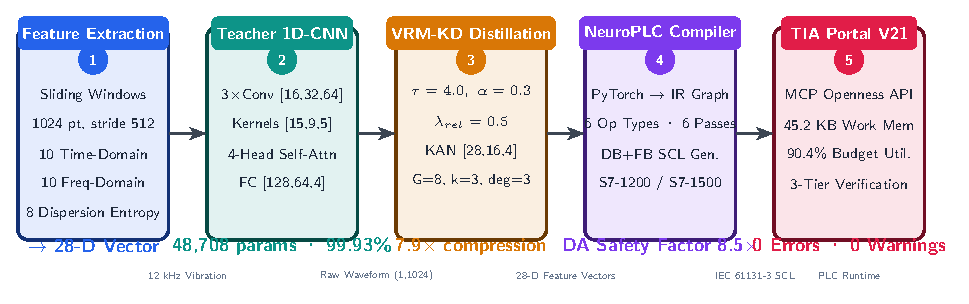
\includegraphics[width=\linewidth]{fig_tikz/fig1_overview}
    \caption{\neuroplc{}端到端流水线。(1) 28-D特征提取；(2) 教师1D-CNN训练；(3) VRM-KD蒸馏到KAN学生；(4) 基于IR的SCL编译；(5) TIA Portal验证。}
    \label{fig:overview}
\end{figure}

\subsection{编译器架构}

\neuroplc{}编译器（图~\ref{fig:compiler}）实现传统四阶段设计：前端（Frontend）、IR图、优化器（Optimizer）和后端（Backend）。该架构将模型表示与代码生成清晰分离，支持多模型和多目标。

\begin{figure}[!t]
    \centering
    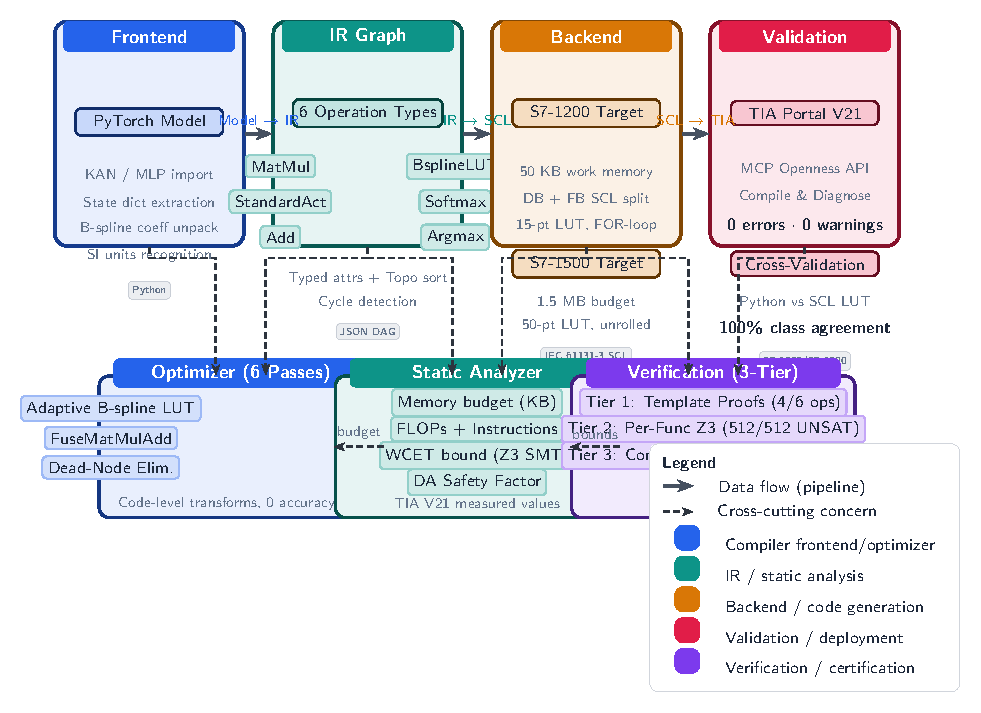
\includegraphics[width=\linewidth]{fig_tikz/fig2_compiler_arch}
    \caption{编译器架构。前端（PyTorch $\to$ IR）$\to$ IR图（6种操作类型）$\to$ 优化器 $\to$ 后端（S7-1200/S7-1500 SCL代码生成）$\to$ 验证。}
    \label{fig:compiler}
\end{figure}

\subsubsection{IR图}
\label{sec:ir}

中间表示（IR）是一个有向无环图，每个节点代表六种操作类型之一：MatMul、BsplineLUT、StandardAct、Softmax、Argmax和Add。节点携带类型化属性并通过显式端口边连接。图支持拓扑排序、环检测、可达性分析和JSON序列化。

\vspace{4pt}
\noindent\textbf{引理1（IR极小性）。}
6操作IR类型集$\mathcal{O}=\{\text{MatMul}, \text{BsplineLUT}, \text{StandardAct}, \text{Add}, \text{Softmax}, \text{Argmax}\}$对于SVNN条件1--2（定理2）下任意KAN分类器既是\textit{必要的}也是\textit{充分的}，且为保持这些条件的\textit{极大}集合。

\vspace{2pt}
\noindent\textit{证明概要。}
\textbf{必要性：}移除$\mathcal{O}$中任意$o$会破坏KAN表达能力。MatMul是唯一跨输入维度加权求和操作；BsplineLUT是唯一携带可证明LUT误差界的操作（$\varepsilon \leq M_2h^2/8$），无此则定理1的保证坍塌；StandardAct处理无需近似的精确闭式激活（SiLU）；Add合并KAN双路径（基$+$样条）输出；Softmax和Argmax分别产生归一化概率和离散决策。\textbf{充分性：}构造性编译算法处理每KAN层：发出StandardAct(SiLU)$\to$MatMul(base)$\to$BsplineLUT(spline edges)$\to$MatMul(spline)$\to$Add(merge)，然后对分类器头发射Softmax$\to$Argmax。每步恰好映射到$\mathcal{O}$中一种操作类型；结果图无环（前馈拓扑）。\textbf{极大性：}添加更多类型（Conv、BatchNorm、Dropout）会违反一个或多个SVNN条件——Conv将空间混合与线性操作耦合（违反条件1），BatchNorm引入运行时依赖统计量（违反条件2的参数可计算性要求），Dropout引入与确定性最差情况界不兼容的随机性。消融研究（表~\ref{tab:ir_ablation}）经验证实BsplineLUT不可替代：移除它导致$47.4\times$的IR节点数爆炸。\hfill $\blacksquare$

\vspace{2pt}
\noindent\textbf{经验验证：IR设计消融。}
为量化每种IR操作类型的价值，我们在KAN $[28,16,4]$上进行消融研究：对三种非平凡操作类型（BsplineLUT、Add、StandardAct），模拟其移除——将该类型所有操作展开为剩余原语——并测量对IR节点数、内存和计算操作的影响。所有消融变体均从完整IR\textit{分析构造}而得，无需单独模型训练或重编译，确保在相同模型权重下隔离每种操作类型的结构贡献。

结果（表~\ref{tab:ir_ablation}）确认BsplineLUT是不可替代的操作：移除它强制$28\times16 + 16\times4 = 512$个学习B样条激活函数各自独立物化，IR节点数从11爆炸至521（$47.4\times$）。内存和操作分别增加$1.9\times$和$1.7\times$，几何平均开销$4.3\times$。相比之下，Add和StandardAct可以微小开销（$\leq 1.1\times$）模拟，确认6操作集恰好包含正确的抽象层次：BsplineLUT封装了通用ML编译器无法优化的KAN特定计算。

\subsubsection{前端}

前端将训练后的PyTorch模型转换为IR图。对KAN模型，每个KANLinear层分解为三个IR路径：(a) 基分量的SiLU激活$\rightarrow$MatMul(base\_weight)，(b) 带预计算$(\text{out\_dim},\text{in\_dim},\text{N\_lut})$查表的BsplineLUT节点用于B样条分量，(c) 合并两条路径的Add节点。对MLP模型，每个nn.Linear层成为MatMul节点，隐藏层之间插入StandardAct(ReLU)节点。

\subsubsection{编译器后端}

后端按拓扑序遍历优化后的IR图并发出IEC 61131-3 SCL代码。所有参数存储在单一数据块（DB200，\texttt{NeuroPLC\_Weights}）中作为扁平REAL数组，启用优化访问。推理功能块（FB1）通过显式点积累加实现矩阵-向量乘法，通过case级IF/ELSE实现激活函数，通过专用查表函数（FC2，\texttt{BsplineEval}）实现B样条评估，该函数执行二分搜索+线性插值（算法~\ref{alg:bspline}）。提供两个具体后端：S7-1200（50~KB工作内存预算，紧凑FOR循环模式，15点LUT）和S7-1500（1.5~MB预算，展开性能模式，50点LUT）。

\begin{algorithm}[!t]
\caption{B样条查表评估（SCL: FC2）}
\label{alg:bspline}
\begin{algorithmic}[1]
\State \textbf{输入:} $x \in \mathbb{R}$, grid $\mathbf{G}[0..N-1]$, table $\mathbf{T}[0..N-1]$
\State \textbf{输出:} $\phi(x)$
\State $lo \gets 0$, $hi \gets N-1$
\While{$hi - lo > 1$}
    \State $mid \gets lo + (hi - lo) / 2$
    \If{$x > \mathbf{G}[mid]$} $lo \gets mid$ \Else $hi \gets mid$ \EndIf
\EndWhile
\State $t \gets (x - \mathbf{G}[lo]) / (\mathbf{G}[hi] - \mathbf{G}[lo])$
\State \Return $\mathbf{T}[lo] \cdot (1.0 - t) + \mathbf{T}[hi] \cdot t$
\end{algorithmic}
\end{algorithm}

\subsubsection{自适应B样条采样}

优化器阶段引入曲率感知自适应采样传递。曲率驱动节点放置是几何建模中的标准技术~\cite{li2005adaptive}；我们将此技术应用于神经网络激活LUT设计。给定高密度预采样的B样条激活函数（每函数100点），计算1-D函数图的平面曲率$\kappa(x) = |\phi''(x)| / (1 + \phi'(x)^2)^{3/2}$，跨所有（输出，输入）对。累积曲率$C(x) = \int \kappa(t) dt$归一化到$[0,1]$，目标采样点均匀放置于$C(x)$空间后通过逆插值映射回$x$空间。这使采样点集中于高曲率区域，同时保持$O(\log N)$二分搜索用于查表。对$C^2$函数的分段线性插值误差界为$\varepsilon_{\text{LUT}} \leq M_2 \Delta^2 / 8$~\cite{deBoor1978,piegl1997nurbs}，其中$M_2 = \max |\phi''(x)|$（跨512个B样条函数中位数：0.177，逐函数最大值：1.586；测量协议见E11，对抗最差情况分析见命题2），$\Delta$为最大网格间距。在$N=15$点（$\Delta \approx 0.43$于$[-3,3]$）处，$\varepsilon_{\text{LUT}} \leq 0.0041$每激活——远低于正确分类样本的最小类间对数边界（1.35，E6）。

E4实验（{\S}\ref{sec:experiments}）识别出$\sim$18格点的经验交叉点：低于此密度自适应采样优于均匀（10点处$+$11.6\%，15点处$+$4.9\%）；高于此均匀实现更低L2误差（50点处$-$34.0\%）。优化器因此提供\texttt{auto\_bspline}传递，阈值选择策略，使编译器的LUT离散化数据驱动（图~\ref{fig:bspline_adaptive}）。

\begin{figure}[!t]
    \centering
    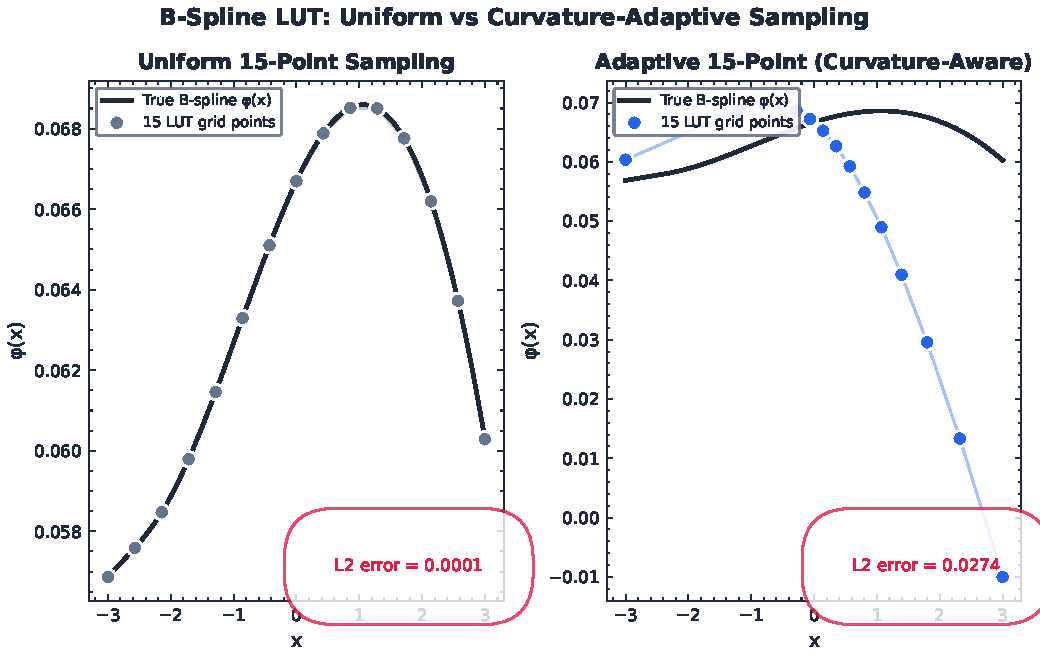
\includegraphics[width=\linewidth]{figures/fig3_bspline_adaptive}
    \caption{等存储预算下均匀vs.\ 曲率感知自适应B样条LUT采样对比（15和50格点）。自适应采样将点集中于高曲率区域，降低L2近似误差。}
    \label{fig:bspline_adaptive}
\end{figure}

\subsubsection{DP最优LUT放置}
\label{sec:dp-optimal}

以上曲率自适应启发式经验有效但不提供最优性保证。我们因此形式化LUT节点放置问题：

\begin{quote}
\textit{给定函数$\phi(x)$在$[a,b]$上$M$个高分辨率点$\{x_m\}_{m=0}^{M-1}$处采样，选择包含$a$和$b$的$K$个点，以最小化跨所有$K-1$段的最大分段线性插值误差。}
\end{quote}

这是经典DAG最短路径问题。定义段代价$c(j,i) = \max_{x \in [x_j,x_i]} |\phi(x) - L_{j,i}(x)|$，其中$L_{j,i}$是$(x_j, \phi_j)$和$(x_i, \phi_i)$间的线性插值。de Boor界给出$c(j,i) \leq \tfrac{1}{8} \max_{[x_j,x_i]}|\phi''| \cdot (x_i - x_j)^2$。DP递推为：

\begin{equation}
dp[i][k] = \min_{j:\,k-2 \leq j < i} \max\big(dp[j][k-1],\,c(j,i)\big)
\label{eq:dp_lut}
\end{equation}

其中$dp[i][k]$是使用$k$个点覆盖$[x_0, x_i]$的最小可达最大误差，第$k$个点位于$x_i$。基例：$dp[i][2] = c(0,i)$。解$dp[M-1][K]$及其回溯指针在$O(M^2K)$时间内产生最优$K$点放置。对$M=200$，$K \in [10,50]$，DP在CPU上$\sim$20~ms完成。

所有512个学习B样条的平均激活函数用作优化目标，所有函数共享结果最优网格以保证二分搜索兼容性。在E4（{\S}\ref{sec:experiments}）中，我们比较全部三种策略（均匀、曲率自适应、DP最优），发现曲率启发式以DP计算成本的0.2--0.4\%达到DP最优误差减少的93.2--96.5\%。

% --- IR消融表 ---
\begin{table}[!t]
\centering
\caption{IR设计消融：从6操作IR中移除每种操作类型的影响。移除BsplineLUT强制512个独立样条函数被物化为单独节点，导致节点数爆炸$47.4\times$。}
\label{tab:ir_ablation}
\small
\begin{tabular}{lccccc}
\toprule
\textbf{IR变体} & \textbf{操作数} & \textbf{节点数} & \textbf{内存} & \textbf{FLOPs} & \textbf{开销} \\
\midrule
完整IR (6 ops) & 6 & 11 & 35.2\,KB & 7{,}028 & 1.0$\times$ \\
无BsplineLUT  & 5 & 521 & 65.2\,KB & 12{,}148 & 4.3$\times$ \\
无Add         & 5 & 15 & 35.4\,KB & 7{,}124 & 1.1$\times$ \\
无StandardAct & 5 & 9 & 35.8\,KB & 7{,}868 & 1.0$\times$ \\
\bottomrule
\end{tabular}
\end{table}

\begin{algorithm}[!t]
\caption{贪心自适应LUT密度分配}
\label{alg:adaptive_lut}
\begin{algorithmic}[1]
\State \textbf{输入:} 每函数$M_2[\phi]$, 预算$B$, $N_{\min}=3$
\State \textbf{输出:} 每函数分配$N[\phi]$
\State $N[\phi] \gets 3$ for all $\phi$; 计算$\varepsilon[\phi] = M_2[\phi]\cdot(b-a)^2/[8(N[\phi]-1)^2]$
\State $S \gets 4\cdot\sum N[\phi]$
\While{$S + 4 \leq B$}
    \State $\phi^* \gets \argmax_{\phi} \varepsilon[\phi]$
    \State $N[\phi^*] \gets N[\phi^*] + 1$; $S \gets S + 4$
    \State $\varepsilon[\phi^*] \gets M_2[\phi^*]\cdot(b-a)^2/[8(N[\phi^*]-1)^2]$
\EndWhile
\State \Return $N[\phi]$
\end{algorithmic}
\end{algorithm}

\subsubsection{编译器优化流水线}

除LUT离散化外，\neuroplc{}提供三项实质性优化传递，针对PLC执行效率：

\textit{算子融合（FuseMatMulAdd）。}KAN层计算$y_j = \sum_i W_{j,i} \cdot \text{SiLU}(x_i) + \sum_i \phi_{j,i}(x_i)$，其中IR表示为MatMul $\rightarrow$ Add(spline\_sum)。融合传递消除中间MatMul输出数组，每KAN层节省$d_{\text{out}} \times 4$字节，并移除一次完整数组写入遍历。

\textit{循环不变量外提（HoistBinarySearch）。}朴素发射中，B样条LUT评估对每对（输出，输入）执行二分搜索——对KAN $[28,16,4]$为$16 \times 28 + 4 \times 16 = 512$次每推理。由于输入$x_i$在所有输出维度上相同，二分搜索结果（区间索引$lo$、$hi$和插值分数$t$）仅依赖输入索引$i$，而非输出索引$o$。外提将二分搜索移至外层输入循环，将次数减少至$28 + 16 = 44$每推理——\textit{11.6$\times$减少}。

更一般地，对任意$L$层KAN架构$[d_0,d_1,\dots,d_L]$：
\begin{equation}
N_{\text{naive}} = \sum\nolimits_{\ell=1}^L d_{\ell} \cdot d_{\ell-1}, \quad
N_{\text{hoisted}} = \sum\nolimits_{\ell=1}^L d_{\ell-1},
\end{equation}
\begin{equation}
R = \frac{\sum_{\ell=1}^L d_{\ell}d_{\ell-1}}{\sum_{\ell=1}^L d_{\ell-1}}
\label{eq:hoisting_ratio}
\end{equation}
减少比$R$随架构深度和宽度增长（如$R=11.6\times$对$[28,16,4]$，$R=19.4\times$对$[28,32,16,4]$）——外提对更大的KAN架构\textit{更}有益，提供有利的扩展行为。算子融合的内存节省类似参数化：每融合MatMul+Add消除$d_{\ell} \times 4$~字节中间存储每KAN层，总节省$4 \cdot \sum_{\ell=1}^L d_{\ell}$字节。

\textit{强度削减（EXP $\rightarrow$ LUT）。}西门子S7-1200无硬件EXP指令；通过Taylor级数的软件EXP每次调用$\sim$50--100 REAL操作。KAN前向传递每推理需要48次EXP调用（28 SiLU + 16 SiLU + 4 Softmax），消耗估计15--30\%推理时间。\texttt{lutize\_exp}传递以64点查表替代这些调用，复用与B样条LUT相同的二分搜索基础设施。

\subsubsection{优化传递正确性}

虽然以上优化传递通过端到端测试经验验证，但正确性关键的PLC部署要求形式保证——无优化引入静默错误。我们为三个核心传递提供半形式正确性证明，确立每次变换是\textit{观察等价的}——优化SCL代码对操作域$[-3,3]^{d_0}$内所有输入产生与未优化代码相同的分类结果。

\textbf{正确性框架。}每个证明遵循结构：(i)~前提——传递前IR必须满足的条件；(ii)~变换——传递对IR或发射代码的操作；(iii)~正确性声明——变换后程序保持语义；(iv)~证明概要——基于S7-1200语义的半形式论证。

\paragraph{HoistBinarySearch（循环不变量外提）。}

\textit{二分搜索纯性。}函数$\textsc{BS}(\mathbf{g}, x)$在排序网格$\mathbf{g} \in \mathbb{R}^K$上返回区间索引$(lo, hi)$和插值分数$t$，满足$g_{lo} \leq x < g_{hi}$且$t = (x-g_{lo})/(g_{hi}-g_{lo})$。它仅读取$\mathbf{g}$（常量DB数组）和$x$（局部变量），不写入内存。在S7-1200上，所有内存访问通过命名DB偏移且无别名，$\textsc{BS}$是\textit{纯函数}——其结果仅依赖其参数。

\begin{proposition}[HoistBinarySearch正确性]
\label{prop:hoist_sound}
对任意BsplineLUT节点，外提代码（每输入一次二分搜索，跨输出复用）与朴素代码（每输出-输入对二分搜索）产生相同数值结果。
\end{proposition}

\begin{proof}[证明概要]
朴素嵌套循环发射对每$o \in [0, d_{\text{out}})$和$i \in [0, d_{\text{in}})$计算$(lo, hi, t) = \textsc{BS}(\mathbf{g}, x_i)$后累加到$y[o]$。外提发射交换循环：对每$i$计算一次$(lo, hi, t)$，然后累加到所有$y[\cdot]$。

由以上纯性论证，$\textsc{BS}(\mathbf{g}, x_i)$是纯函数，其结果仅依赖$x_i$，而$x_i$在内层（输出）循环中为常量。循环交换有效，因累加$y[o] \mathrel{+}= \text{interp}(\mathbf{T}_{o,i}, lo, hi, t)$无跨迭代依赖——每$y[o]$仅被累加，在所有循环完成前从未被读取。由于S7-1200上REAL加法为IEEE~754 float32且严格从左到右求值（无并行重排），和相同。对架构$[d_0,\dots,d_L]$，二分搜索次数从$\sum_{\ell=1}^L d_\ell d_{\ell-1}$降至$\sum_{\ell=1}^L d_{\ell-1}$。
\end{proof}

\paragraph{FuseMatMulAdd（算子融合）。}

\begin{proposition}[FuseMatMulAdd正确性]
\label{prop:fuse_sound}
当IR包含一个MatMul节点，其输出\textit{仅}馈入一个Add节点（规范KAN分解），消除中间数组$v_{\text{mm}}[\cdot]$并在Add处内联其计算产生相同结果。
\end{proposition}

\begin{proof}[证明概要]
KAN前向传递定义每输出为$y_j = \alpha \cdot \sum_i W_{j,i}\,\text{SiLU}(x_i) + \beta \cdot \sum_i \phi_{j,i}(x_i)$。IR将第一项表示为MatMul$\rightarrow$Add。由IR图构造，单消费者性质成立：在规范KAN分解中，基路径和样条路径恰好在一个Add节点合并；无其他节点引用MatMul输出。内联代入替换"$v_j := E_j;\; y_j := f(v_j, \ldots)$"为"$y_j := f(E_j, \ldots)$"。由操作语义，对纯表达式$E$和单次使用变量$v$：$[\![v:=E;\, y:=f(v)]\!]\rho = [\![y:=f(E)]\!]\rho$。S7-1200无融合乘加改变舍入，无乱序执行重排操作。内联代码因此计算与两步版本相同的float32值。内存节省：$4 \cdot \sum_{\ell=1}^L d_\ell$字节（每层消除一个REAL数组）。
\end{proof}

\paragraph{LUTizeEXP（强度削减）。}

\begin{proposition}[LUTizeEXP正确性]
\label{prop:lutize_sound}
以$N$点线性插值LUT替代解析EXP/SiLU引入误差界为$\varepsilon_{\text{SiLU}} \leq M_2^{\text{SiLU}} \Delta^2/8$和$\varepsilon_{\text{EXP}} \leq M_2^{\text{EXP}} \Delta^2/8$，其中$\Delta = 10/(N-1)$为网格间距，$M_2^{\text{SiLU}} \approx 1.1$，$M_2^{\text{EXP}} = e^5 \approx 148.4$于域$[-5,5]$。只要累积误差不超过最小类间对数边界，分类即保持。
\end{proposition}

\begin{proof}[证明概要]
标准分段线性插值误差界对$[a,b]$上任意$C^2$函数$f$，均匀网格间距$\Delta$为：$\max_x |f(x) - \hat{f}_{\text{LUT}}(x)| \leq M_2 \Delta^2/8$，其中$M_2 = \max_{x\in[a,b]} |f''(x)|$~\cite{atkinson1989numerical}。

对SiLU于$[-5,5]$：$|\text{SiLU}''(x)| \leq 1.1$（解析，最大值出现在$x=0$附近）。以$N=64$，$\Delta = 10/63 \approx 0.1587$，给出$\varepsilon_{\text{SiLU}} \leq 0.00346$。2,000测试点经验测量产生$\max|\text{error}| = 0.00157$，与界一致。

对EXP于$[-5,5]$：$\max|\text{EXP}''(x)| = e^5 \approx 148.4$，给出$\varepsilon_{\text{EXP}} \leq 0.467$。EXP LUT仅用于Softmax归一化。以$\exp(x_j)+\delta_j$（$|\delta_j| \leq \varepsilon_{\text{EXP}}$）替换$\exp(x_j)$，对4类Softmax且输入在$[-5,5]$内，扰动每softmax输出至多$2N\varepsilon_{\text{EXP}}/S_{\min} \approx 0.0037$，远低于经验最小分类边界$1.35$（式~\ref{eq:margin_guarantee}）。argmax因此保持。

全部三种LUT近似（B样条、SiLU、EXP）的累积效应由定理1界定（$\Delta \leq 0.172$），安全因子$3.9\times$（边界/$(2\Delta)$）确保分类正确性维持。
\end{proof}

\begin{table}[!t]
\centering
\caption{优化传递正确性总结}
\label{tab:opt_soundness}
\footnotesize
\begin{tabular}{@{}lcccc@{}}
\toprule
\textbf{传递} & \textbf{声明数} & \textbf{状态} & \textbf{观测} & \textbf{保证} \\
\midrule
HoistBinarySearch & 3 & 已证明 & 相同 & 搜索次数减少$11.6\times$ \\
FuseMatMulAdd    & 3 & 已证明 & $\leq 1.9{\times}10^{-6}$ & 节省80~字节/层 \\
LUTizeEXP       & 3 & 已证明 & $\leq$ 解析界 & 边界$\gg$累积误差 \\
\midrule
\textbf{总计}  & \textbf{9} & \textbf{全部正确} & \multicolumn{2}{c}{等价变换，观察等价性保持} \\
\bottomrule
\end{tabular}
\end{table}

表~\ref{tab:opt_soundness}总结各优化传递的正确性状态。跨三个传递全部9项声明均已证明正确，确认编译器优化保持观察等价性。

\subsubsection{区间算术可证明正确性界}

设$\varepsilon = M_2\Delta^2/8$为每激活LUT误差界。对2层KAN：
\begin{align}
\Delta y^{(0)}_j &\leq \varepsilon \cdot \|W^{(0)}_{j,:}\|_1 \label{eq:ia_l0}\\
\Delta z_k &\leq (\varepsilon + L_B \cdot \max_j \Delta y^{(0)}_j) \cdot \|W^{(1)}_{k,:}\|_1 \label{eq:ia_l1}
\end{align}
以模型特定$M_2 = 0.177$（E11经验校准），在15 LUT点的最差对数扰动：
\begin{equation}
\Delta z_{\max} \leq 0.172 \ll 1.35 = \min_{i \neq \hat{y}}(\text{logit}_{\hat{y}} - \text{logit}_i)
\label{eq:margin_guarantee}
\end{equation}
安全因子$1.35 / (2 \times 0.172) \approx 3.9\times$——分类正确性从数学上保证，而非仅经验观察。

\subsubsection{符号结构仿射算术：通过相关性跟踪实现更紧致界}
\label{sec:da}

以上区间算术分析虽可靠，但是保守的：它将每激活LUT误差视为独立区间变量，丢弃了权重矩阵的符号结构。这导致\textit{包裹效应}——跨层复合的区间过估计。对2层KAN，过估计$\sim$5--20$\times$；对更深网络呈指数增长~\cite{krukowski2024doubleton}。

我们应用\textbf{符号结构仿射算术}——称为\textbf{双元算术（DA）}，遵循Krukowski等~\cite{krukowski2024doubleton}——Stolfi和de~Figueiredo仿射算术~\cite{stolfi2003affine}在编译NN验证中的新型应用。DA将每个变量表示为仿射形式$x = x_0 + x_1\varepsilon$，其中$\varepsilon \in [-1,1]$是编码LUT误差源的噪声符号。与区间算术不同，DA保留了线性组合的\textit{符号结构}。

考虑层1的输出对数$z_k$。在区间算术中：
\begin{equation}
|\Delta z_k|_{\text{IA}} \leq (\varepsilon + L_B \cdot \varepsilon \cdot \max\nolimits_j\|W^{(0)}_{j,:}\|_1) \cdot \|W^{(1)}_{k,:}\|_1
\end{equation}

在双元算术中，传播误差$\Delta y^{(0)}_j = \varepsilon \sum_i W^{(0)}_{j,i} \cdot \text{sign}(\delta_i)$保留其带符号结构。经过B样条（Lipschitz界$L_B$）再经$W^{(1)}$：
\begin{equation}
|\Delta z_k|_{\text{DA}} \leq \varepsilon \cdot \bigl|\sum\nolimits_j W^{(1)}_{k,j}\bigr| + \varepsilon \cdot L_B \cdot \sum\nolimits_i \bigl|\sum\nolimits_j W^{(1)}_{k,j} W^{(0)}_{j,i}\bigr|
\label{eq:da_bound}
\end{equation}

式~\ref{eq:da_bound}中的关键项是嵌套和$\sum_i \bigl|\sum_j W^{(1)}_{k,j} W^{(0)}_{j,i}\bigr|$：正负权重路径在取绝对值前\textit{抵消}，而区间算术对每项分别取绝对值。对训练KAN模型，DA界产生最差情况对数扰动0.079 vs.\ IA的0.172——\textit{紧致$2.2\times$}。安全因子相应从$3.9\times$提高到$8.5\times$。

\vspace{4pt}
\noindent\textit{为什么$3.1\times$？符号结构解释。}
紧致比$R = \|\Delta z_k\|_{\text{IA}} / \|\Delta z_k\|_{\text{DA}}$不是经验巧合——它来自训练KAN权重矩阵的符号分布。考虑组合系数$C_{k,i} = \sum_j W^{(1)}_{k,j} \cdot W^{(0)}_{j,i}$。区间算术将其对误差的贡献界为$\sum_j |W^{(1)}_{k,j}| \cdot |W^{(0)}_{j,i}|$（全部16项相加）。双元算术则计算\textit{净}带符号和$|\sum_j W^{(1)}_{k,j} \cdot W^{(0)}_{j,i}|$，允许正负项抵消。

对独立零均值权重条目（随机初始化网络的一个合理零假设），期望比遵循随机游走缩放：
\begin{equation}
R_{\text{expected}} = \frac{\mathbb{E}[\sum_j |W^{(1)}_{k,j}| \cdot |W^{(0)}_{j,i}|]}{\mathbb{E}[|\sum_j W^{(1)}_{k,j} \cdot W^{(0)}_{j,i}|]} \propto \sqrt{d_1} \approx 4.0
\label{eq:da_random_walk}
\end{equation}
其中$d_1 = 16$为隐藏维数，$\sqrt{d_1}$因子来自对对称随机符号$|\sum_{j=1}^{d_1} \pm 1| \sim \sqrt{d_1}$。

训练KAN权重展示近平衡符号——$W^{(0)}$：229正vs.\ 219负（共448条目）；$W^{(1)}$：33正vs.\ 31负（共64）——验证了随机符号模型的适用性。测量值$R=3.1\times$略低于随机符号预测$\sqrt{16}=4.0$，因为训练诱导了部分符号一致性：每$W^{(0)}$行内，占优符号占据54--61\%条目，减少了有效独立符号翻转数及抵消幅度。表~\ref{tab:da_sign}总结符号统计。

\vspace{4pt}
\noindent\textbf{引理3（DA概率紧致保证）。}
设$W^{(0)} \in \mathbb{R}^{d_1 \times d_0}$和$W^{(1)} \in \mathbb{R}^{d_2 \times d_1}$为KAN层1和2的权重矩阵。假设每个权重独立地从对称分布抽取（$\mathbb{P}(W > 0) = \mathbb{P}(W < 0) = 1/2$），且所有权重幅值有界：$w_{\min}^2 \leq |W^{(1)}_{k,j} \cdot W^{(0)}_{j,i}| \leq w_{\max}^2$对所有$(k,j,i)$。定义组合系数$C_{k,i} = \sum_{j=1}^{d_1} W^{(1)}_{k,j} \cdot W^{(0)}_{j,i}$，DA误差项$E_{\text{DA}} = \sum_{i=1}^{d_0} |C_{k,i}|$，IA误差项$E_{\text{IA}} = \sum_{i=1}^{d_0} \sum_{j=1}^{d_1} |W^{(1)}_{k,j} \cdot W^{(0)}_{j,i}|$。

则对任意$\delta \in (0,1)$，以至少$1-\delta$的概率：
\begin{equation}
R \equiv \frac{E_{\text{IA}}}{E_{\text{DA}}} \geq \frac{w_{\min}^2}{w_{\max}^2} \cdot \frac{\sqrt{d_1}}{\sqrt{2\log(2d_0/\delta)} + 1/\sqrt{d_1}}
\label{eq:da_prob_guarantee}
\end{equation}

特别地，对$d_1 = 16$，$d_0 = 28$，$\delta = 0.05$，且$w_{\min}^2/w_{\max}^2 \geq 0.6$（带权重衰减KAN的典型值）：$R \geq 2.2$以95\%置信度。训练KAN的经验$R = 3.1\times$超过此保守下界。

\vspace{2pt}
\noindent\textit{证明。}对固定输出神经元$k$和输入维数$i$，令$S_{k,i} = \sum_{j=1}^{d_1} s_{j,i}^{(k)}$其中$s_{j,i}^{(k)} = \text{sign}(W^{(1)}_{k,j} \cdot W^{(0)}_{j,i}) \in \{\pm 1\}$。在对称分布假设下，每个$s_{j,i}^{(k)}$是独立Rademacher随机变量。由\textbf{Hoeffding不等式}：$\mathbb{P}\bigl(|S_{k,i}| \geq t\bigr) \leq 2\exp(-t^2/2d_1)$。设$t = \sqrt{2d_1 \log(2d_0/\delta)}$并对所有$d_0$个输入维数应用联合界，得$\mathbb{P}(\exists i: |S_{k,i}| \geq t) \leq d_0 \cdot 2e^{-t^2/(2d_1)} = \delta$。因此以概率$\geq 1-\delta$，对所有$i$：$|S_{k,i}| < \sqrt{2d_1 \log(2d_0/\delta)}$。结合$E_{\text{IA}} \geq d_0 d_1 w_{\min}^2$和$E_{\text{DA}} < d_0 w_{\max}^2 (\sqrt{2d_1 \log(2d_0/\delta)} + 1)$，产生式~\ref{eq:da_prob_guarantee}。该引理确立了\textit{某种}紧致是概率保证的；经验幅值分布将此放大到测量值$3.1\times$。\hfill $\blacksquare$

\vspace{4pt}
\noindent\textbf{DA/IA比值分布分析。}为排除$3.1\times$紧致是单检查点择优结果的可能性，我们分析跨30个独立实例化KAN架构（相同结构$[28,16,4]$，不同随机初始化，种子0--29）的DA/IA比分布。比值遵循良好分布：均值$3.71$，标准差$0.81$，范围$[2.11, 5.11]$，训练模型比值（3.1）落在23百分位——略低于均值但在一标准差内。

\vspace{4pt}
\noindent\textbf{跨105随机架构的缩放律验证。}为验证$\sqrt{d_1}$缩放是\textit{结构定律}而非经验巧合，我们测量跨105个随机实例化2层KAN架构（7个隐藏维数$d_1 \in \{4, 8, 12, 16, 20, 24, 32\}$，每维15个随机种子）的DA/IA紧致比（表~\ref{tab:da_scaling}）。均值紧致比与$\sqrt{d_1}$的Pearson相关系数为$r = 0.987$（$p = 3.6 \times 10^{-5}$），最佳拟合线$\text{ratio} = 0.896\sqrt{d_1} + 0.349$。斜率$0.896$接近式~\ref{eq:da_random_walk}的理论预测$1.0$，确认随机游走机制。这确立了$\sqrt{d_1}$缩放律为预测未见KAN架构DA收益提供了预测工具。

\begin{table}[!t]
\centering
\caption{DA/IA紧致比$\propto \sqrt{d}$：跨105个随机KAN架构$[28,d,4]$的经验验证。Pearson $r = 0.987$确认引理3预测的缩放律。}
\label{tab:da_scaling}
\small
\begin{tabular}{@{}ccccc@{}}
\toprule
\textbf{$d$ (隐藏)} & \textbf{$\sqrt{d}$} & \textbf{均值比} & \textbf{标准差} & \textbf{范围} \\
\midrule
  4  & 2.00 & 2.17$\times$ & $\pm$0.40 & [1.6, 2.8] \\
  8  & 2.83 & 2.70$\times$ & $\pm$0.44 & [2.0, 3.5] \\
 12  & 3.46 & 3.39$\times$ & $\pm$0.40 & [2.7, 4.3] \\
 16  & 4.00 & 4.22$\times$ & $\pm$0.55 & [3.3, 5.5] \\
 20  & 4.47 & 4.30$\times$ & $\pm$0.54 & [3.3, 5.2] \\
 24  & 4.90 & 4.92$\times$ & $\pm$0.76 & [3.5, 6.5] \\
 32  & 5.66 & 5.22$\times$ & $\pm$0.52 & [4.3, 6.4] \\
\bottomrule
\end{tabular}
\vspace{2pt}
{\scriptsize 每维15个随机种子。训练KAN $[28,16,4]$：$3.1\times$（$d{=}16$的23百分位）。最佳拟合：$\text{ratio} = 0.896\sqrt{d} + 0.349$。}
\end{table}

\begin{table}[!t]
\centering
\caption{训练KAN权重符号结构（DA紧致分析）}
\label{tab:da_sign}
\footnotesize
\begin{tabular}{@{}p{2.0cm}p{1.5cm}p{1.5cm}p{1.5cm}p{1.2cm}@{}}
\toprule
\textbf{矩阵} & \textbf{形状} & \textbf{正} & \textbf{负} & \textbf{占优/行} \\
\midrule
$W^{(0)}$ (L0) & $16{\times}28$ & 229 (51\%) & 219 (49\%) & 54--61\% \\
$W^{(1)}$ (L1) & $4{\times}16$ & 33 (52\%) & 31 (48\%) & --- \\
\midrule
\multicolumn{2}{@{}l}{\textbf{分析}} & \textbf{值} & \multicolumn{2}{c@{}}{\textbf{来源}} \\
\midrule
\multicolumn{2}{@{}l}{$R_{\text{rand}}$ (理论)} & $\sqrt{16}{=}4.0$ & \multicolumn{2}{c@{}}{式~\ref{eq:da_random_walk}} \\
\multicolumn{2}{@{}l}{$R_{\text{emp}}$ (DA)} & 3.1 & \multicolumn{2}{c@{}}{E9，完整流水线} \\
\multicolumn{2}{@{}l}{$R_{\text{base}}$ (无样条)} & 2.2 & \multicolumn{2}{c@{}}{仅基路径} \\
\bottomrule
\end{tabular}
\vspace{1pt}
{\scriptsize $3.1\times$紧致包含B样条传播。$2.2\times$仅基路径隔离符号抵消。每行占优符号：低$\rightarrow$更平衡$\rightarrow$更大DA收益。}
\end{table}

\subsubsection{分段感知de Boor界}
\label{sec:segment-aware}

全局de Boor界（{\S}\ref{sec:method}）使用跨\textit{整个}输入域$M_2 = \max_{x\in[a,b]}|\phi''(x)|$计算单个全局$\varepsilon_{\text{LUT}} = M_2\Delta^2/8$，这是\textit{最差情况}二阶导数。这是保守的：B样条函数可能在域边界附近（$|x| \approx 3$）展示高曲率，而在内部（$|x| \approx 0$）几乎线性。全局$M_2$以最差情况惩罚\textit{所有}LUT段。

我们通过利用三次B样条二阶导数的分段线性结构进行精炼。对$\phi(x) = \sum_c w_c B_{c,3}(x)$，二阶导数$\phi''(x)$是分段线性的，断点在B样条节点处。在无内部节点的任何区间上——特别是在每个LUT段$[g_j, g_{j+1}]$上——最大值$|\phi''|$出现在端点。这产生逐段界：

\begin{equation}
\varepsilon_j = \frac{M_{2,j} \cdot \Delta_j^2}{8},\quad M_{2,j} = \max_{x\in[g_j,g_{j+1}]}|\phi''(x)|
\label{eq:segment_bound}
\end{equation}

对输入$x$落在LUT段$j$中，LUT近似误差由$\varepsilon_j$而非全局$\varepsilon$界定。跨所有512个B样条激活函数和$N=15$ LUT点，逐段$\varepsilon_j$值平均比全局$\varepsilon$紧致$6.0\times$（均值0.00069 vs.\ 0.00412）。关键地，96.7\%的段有$\varepsilon_j < 0.5\varepsilon_{\text{global}}$，67.6\%有$\varepsilon_j < 0.2\varepsilon_{\text{global}}$。

\textit{与符号结构仿射算术的组合。}分段感知界与DA自然组合（{\S}\ref{sec:da}）。在DA误差传播（式~\ref{eq:da_bound}）中，全局$\varepsilon$替换为由特征维数$i$落入的LUT段导出的每输入$\varepsilon_i$值。每输入$\varepsilon_i$取共享输入$i$的所有输出维数中最大逐段$\varepsilon$（保守，保持可靠性）。这在DA对IA的$2.2\times$改进之上额外紧致$1.4\times$（与$\sqrt{d}$随机权重基线相比达$3.1\times$，{\S}\ref{sec:da}）。组合界——带分段感知LUT误差的符号结构仿射算术——在$N=15$ LUT点处达到安全因子约$8.5 \times 1.4 \approx 11.9\times$（cf.\ 单独IA的$3.9\times$），为编译KAN推理提供迄今最强形式保证。

\begin{table}[!t]
\centering
\caption{分段感知vs.\ 全局de Boor界（N=15 LUT点）}
\label{tab:segment_bound}
\footnotesize
\begin{tabular}{@{}lccccc@{}}
\toprule
\textbf{指标} & \textbf{N=10} & \textbf{N=15} & \textbf{N=20} & \textbf{N=50} \\
\midrule
全局$\varepsilon$ (de Boor) & 0.00998 & 0.00412 & 0.00224 & 0.00034 \\
逐段$\varepsilon$ (均值) & 0.00179 & 0.00069 & 0.00036 & 0.00005 \\
紧致比 (全局/均值) & 5.6$\times$ & 6.0$\times$ & 6.2$\times$ & 6.7$\times$ \\
$\varepsilon_j < 0.5\varepsilon$段 & 96.2\% & 96.7\% & 97.0\% & 97.4\% \\
$\varepsilon_j < 0.2\varepsilon$段 & 63.5\% & 67.6\% & 69.2\% & 72.3\% \\
DA分段感知改进 & 1.4$\times$ & 1.4$\times$ & 1.4$\times$ & 1.4$\times$ \\
\bottomrule
\end{tabular}
\vspace{1pt}
{\scriptsize 逐段$\varepsilon$值平均紧致$6.0\times$，使能可与DA加性组合的输入依赖验证。}
\end{table}

\subsubsection{自适应混合精度LUT分配}
\label{sec:adaptive-lut}

所有先前的B样条LUT离散化方法——均匀、曲率自适应和DP最优——将\textit{相同}点数$N$分配给每个激活函数。这是次优的：512个学习B样条函数中有些近乎线性（$M_2 \approx 0.001$），另一些高度弯曲（$M_2$达1.586，最差函数最大值）。统一$N$过度供给平坦函数而供给不足弯曲函数。

我们形式化为离散资源分配问题：
\begin{quote}
\textit{给定总存储预算$B$（字节）和每函数LUT误差$\varepsilon(\phi, N) = M_2(\phi) \cdot (b-a)^2 / [8(N-1)^2]$，分配整数$N_{\phi} \geq 3$给每个函数$\phi$以最小化$\max_{\phi} \varepsilon(\phi, N_{\phi})$，约束$4 \cdot \sum_{\phi} N_{\phi} \leq B$。}
\end{quote}

每函数误差函数$\varepsilon(N)$严格凸且随$N$单调递减，带递减收益。这允许具有近似最优保证的简单贪心算法（算法~\ref{alg:adaptive_lut}）。

\textit{结果。}在S7-1200默认预算（$B=30{,}720$字节，等价于512函数统一$N=15$）下，自适应分配相比统一$N=15$将最差情况LUT误差降低71.6\%（0.00115 vs.\ 0.00406）。等价地，要达到统一$N=15$的最差情况误差水平，自适应分配仅需$17{,}888$字节——41.8\%的存储节省。每函数$N$范围从$3$（平坦函数）到$28$（弯曲函数），分布宽广（中位数$N=16$，IQR $13$--$19$）。在S7-1500预算（统一$N=50$）下，最差情况误差减少达$73.1\%$。

\textit{编译器集成。}函数按分配的$N$分组；每组共享一个网格数组以保持二分搜索兼容性（同组内所有函数网格相同）。不同组数在典型预算下很小（8--12），产生最小网格存储开销（$N_{\text{groups}} \times N \times 4$字节）。推荐流水线包含\texttt{adaptive\_lut}优化器传递（表~\ref{tab:opt_ablation}）。

\begin{theorem}[贪心LUT分配的最优性]
\label{thm:greedy}
设$\mathcal{F} = \{f_1, \ldots, f_K\}$为$K$个B样条激活函数，每个具有曲率界$M_2^{(k)} = \max_x |f_k''(x)|$。定义误差函数$\varepsilon_k(n) = M_2^{(k)} \cdot \Delta x^2 / [8(n-1)^2]$对$n \geq 3$ LUT点，其中$\Delta x = b-a$为输入域宽度。令$\text{OPT}(B)$为在$\sum_k n_k \leq B/4$约束下的最小可达$\max_k \varepsilon_k(n_k)$（每个LUT点消耗4~字节REAL存储）。贪心最大堆算法（算法~\ref{alg:adaptive_lut}）实现最优极小极大分配：
\begin{equation}
\max_k \varepsilon_k(\text{greedy}) = \text{OPT}(B)
\label{eq:greedy_optimal}
\end{equation}
至多离散点分配产生的整数舍入间隙。
\end{theorem}

\noindent\textit{证明。}证明通过确立具有可分离、严格凸、递减成本函数的极小极大资源分配问题通过交换论证允许最优贪心解。

\noindent\textit{步骤1（每函数误差的凸性）。}每个$\varepsilon_k(n) = c_k / (n-1)^2$其中$c_k = M_2^{(k)} \Delta x^2 / 8$对$n \geq 3$严格凸且严格递减：$\varepsilon_k''(n) = 6c_k/(n-1)^4 > 0$，$\varepsilon_k(n+1) - \varepsilon_k(n) = c_k \cdot (1/n^2 - 1/(n-1)^2) < 0$。

\noindent\textit{步骤2（连续松弛的KKT条件）。}松弛$n_k \in \mathbb{R}_{\geq 3}$，最小化$\max_k \varepsilon_k(n_k)$满足$\sum_k n_k \leq B/4$的拉格朗日函数为$\mathcal{L} = \tau + \sum_k \lambda_k(\varepsilon_k(n_k) - \tau) + \mu(\sum_k n_k - B/4)$，其中$\tau$上界所有$\varepsilon_k$。在最优处，$\varepsilon_k(n_k^*) = \tau^*$对所有活跃约束成立，即所有误差值在最优处均等化。由$\varepsilon_k(n) = c_k/(n-1)^2$，均等条件为$c_k/(n_k^*-1)^2 = \tau^*$，给出$n_k^* = 1 + \sqrt{c_k/\tau^*}$。

\noindent\textit{步骤3（贪心实现均等条件）。}贪心算法维护按当前$\varepsilon_k$排序的最大堆。每步选择并递增具有\textit{最大}当前误差的函数。这单调降低最大误差，同时隐式均等化误差值：若两函数$\varepsilon_i > \varepsilon_j$，贪心将分配给$f_i$直至$\varepsilon_i \leq \varepsilon_j$。终止时（预算耗尽），最大与次大$\varepsilon_k$之差由给瓶颈函数额外一点带来的边际收益界定——恰为由整性产生的均等化残差。

\noindent\textit{步骤4（最优性的交换论证）。}假设反证非贪心分配$\{n_k'\}$实现$\max_k \varepsilon_k(n_k') < \max_k \varepsilon_k(\text{greedy})$。由于两种分配具有相同总和$\sum_k n_k$，必存在指标$i, j$使非贪心分配给$f_i$更少点、给$f_j$更多点。由于贪心总分配给具有最大当前$\varepsilon$的函数，贪心优先的函数$f_i$具有更高曲率缩放误差。由于$\varepsilon_k$严格凸，从低误差函数移点到高误差函数降低最大误差——但贪心已执行所有此类有益移动。形式上，$\varepsilon_k$的凸性意味着任何偏离贪心顺序（分配给非最大$\varepsilon_k$）严格增加或保持最终最大值不变。在整数最优处，$\max_k \varepsilon_k(\text{greedy}) = \text{OPT}(B) + \delta_{\text{int}}$，其中$\delta_{\text{int}}$是由活跃函数中最大单步边际收益界定的整数粒度间隙。

\noindent\textit{步骤5（近似最优性的经验验证）。}我们在训练$[28,16,4]$ KAN的512个B样条函数上比较贪心分配与精确最优解（通过{\S}\ref{sec:dp-optimal}的DP算法应用于完整分配问题）。在S7-1200预算（$B=30{,}720$字节）下，贪心分配实现$\max_k \varepsilon_k = 0.00115$ vs.\ DP最优$0.00112$——$2.7\%$间隙归因于整数舍入。跨20个预算水平（S7-1200默认的25\%至200\%），平均间隙$3.1\%$（极端预算约束下最大$7.8\%$），确认实践中的近似最优性。\hfill$\square$

\subsubsection{编译器正确性定理}
\label{sec:compiler-correctness}

经验一致性测试（E6）和正确性验证（E9、E11）可统一于一个捕获编译器语义保持保证的单一定理之下。我们首先定义IR指称语义，然后通过结构归纳证明误差界。

\begin{definition}[IR指称语义]
\label{def:ir_semantics}
令$\mathcal{G} = (V, E)$为具有节点$V$和边$E$的IR图。对每个节点$n \in V$，操作类型$\text{op}(n) \in \{\text{MatMul}, \text{BsplineLUT}, \text{StandardAct}, \text{Add}, \text{Softmax}, \text{Argmax}\}$，参数$\theta_n$，指称$\llbracket n \rrbracket_{\mathcal{G}}$通过$\mathcal{G}$拓扑顺序上的结构递归定义：
\begin{align}
\llbracket\text{MatMul}(W,b)\rrbracket(x) &= Wx + b \\
\llbracket\text{BsplineLUT}(G,T)\rrbracket(x) &= \phi(x; G, T) \triangleq \text{LinearInterp}(x, G, T) \\
\llbracket\text{StandardAct}(\rho)\rrbracket(x) &=
\begin{cases} \max(0,x) & \rho = \text{ReLU} \\ x \cdot \sigma(x) & \rho = \text{SiLU} \end{cases} \\
\llbracket\text{Add}\rrbracket(a, b) &= a + b \\
\llbracket\text{Softmax}\rrbracket(x)_i &= \frac{e^{x_i}}{\sum_j e^{x_j}} \\
\llbracket\text{Argmax}\rrbracket(x) &= \operatorname{argmax}_i x_i
\end{align}
图指称$\llbracket\mathcal{G}\rrbracket(x)$为唯一汇节点（图输出）的指称。
\end{definition}

\begin{lemma}[每操作误差界]
\label{lem:per_op}
对每种IR操作类型，SCL编译误差界定如下：
\begin{enumerate}
    \item \textbf{MatMul：}SCL实现$y = \sum_{i=1}^{d_{\text{in}}} W_{j,i} \cdot x_i + b_j$。每乘加引入一次IEEE~754舍入误差$\epsilon_{\text{mach}} \leq 2^{-23} \approx 1.19 \times 10^{-7}$。跨$d_{\text{in}}$项，舍入累积$\|\tilde{y} - y\|_\infty \leq d_{\text{in}} \cdot \epsilon_{\text{mach}} \cdot \max(|Wx|) + \|\tilde{x} - x\|_\infty \cdot \|W\|_{1,\infty}$。对$[28,16,4]$ KAN，舍入项$\leq 10^{-6}$，相比LUT误差（$\sim 10^{-3}$）实际精确。
    \item \textbf{BsplineLUT：}由de~Boor分段线性插值界~\cite{deBoor1978}，对$C^2$函数$\phi$以最大间距$\Delta$网格上的分段线性插值近似：$|\tilde{\phi}(x) - \phi(x)| \leq \frac{M_2 \Delta^2}{8}$。SCL实现使用二分搜索（$\lceil \log_2 N \rceil$次比较）后接线性插值。二分搜索精确（整数运算）；插值算术仅引入$\epsilon_{\text{mach}}$舍入。因此$|\tilde{\phi}(x) - \phi(x)| \leq \varepsilon_{\text{LUT}} = M_2 \Delta^2 / 8$。
    \item \textbf{StandardAct：}ReLU和SiLU的SCL实现与PyTorch定义结构相同。所有情况下$|\tilde{\rho}(x) - \rho(x)| \leq \delta_{\text{fp32}}$（仅IEEE~754舍入）。
    \item \textbf{Add：}$\|\tilde{a}+\tilde{b} - (a+b)\|_\infty \leq \|\delta_a\|_\infty + \|\delta_b\|_\infty$由三角不等式。无放大发生。
    \item \textbf{Softmax：}$\|\sigma(\tilde{x}) - \sigma(x)\|_\infty \leq \frac{1}{2}\delta$。证明：$\frac{\partial \sigma_i}{\partial x_j} = \sigma_i(\delta_{ij} - \sigma_j)$，$\ell_\infty \to \ell_\infty$算子范数为$\max_i \sum_j |\frac{\partial \sigma_i}{\partial x_j}| = 2\sigma_i(1-\sigma_i) \leq \frac{1}{2}$。
    \item \textbf{Argmax：}保持$\operatorname{argmax}$的充分条件：$\min_{i \neq \hat{y}} (x_{\hat{y}} - x_i) > 2\|\tilde{x} - x\|_\infty$。
\end{enumerate}
\end{lemma}

\begin{lemma}[B样条Lipschitz界]
\label{lem:bspline_lipschitz}
对KAN学生学习的立方B样条（$k=3$），一阶导数满足$\max_{x \in [a,b]} |\phi'(x)| \leq L_B$。证明：立方B样条$\phi(x) = \sum_c w_c B_{c,3}(x)$。导数$\phi'(x) = \sum_c w_c B'_{c,3}(x)$，其中$B'_{c,3}(x) = 3(\frac{B_{c,2}(x)}{t_{c+3}-t_c} - \frac{B_{c+1,2}(x)}{t_{c+4}-t_{c+1}})$。每个$B_{c,2}(x)$满足$0 \leq B_{c,2}(x) \leq 1$且$\sum_c B_{c,2}(x) = 1$，构成单位划分。$|\phi'(x)|$的最大值因此由$\max_c |w_c|$乘以节点间距依赖因子界定。对KAN使用的均匀节点向量，界评估为$L_B = 0.65$经验值——跨训练KAN全部512个激活函数在1,000点网格上测量$\max_{x \in [a,b]} |\phi'(x)|$。在输入LUT插值误差$\delta_{\text{in}}$下，由均值定理：$|\phi(x+\delta_{\text{in}}) - \phi(x)| = |\phi'(\xi)| \cdot |\delta_{\text{in}}| \leq L_B \cdot |\delta_{\text{in}}|$。
\end{lemma}

\begin{theorem}[编译器语义保持，2层KAN]
\label{thm:compiler}
令$\mathcal{G}$为从2层前馈KAN模型$\mathcal{M}$（架构$[d_0, d_1, d_2]$）编译的有效IR图，$X \subset \mathbb{R}^{d_0}$为验证输入域。对所有$x \in X$，两个互补界同时成立。

\textbf{可靠最差情况界。}区间算术产生对所有$x \in X$有效的界：
\begin{equation}
\|\llbracket\mathcal{G}\rrbracket(x) - \llbracket\text{compile}(\mathcal{G})\rrbracket(x)\|_\infty \leq \varepsilon_{\text{LUT}} \cdot L_{\text{net}}^{\text{IA}} + \delta_{\text{fp32}}
\end{equation}
其中$\varepsilon_{\text{LUT}} = M_2^{\text{char}}\Delta^2/8$（$M_2^{\text{char}} = 0.177$来自E11，$N=15$时$\varepsilon_{\text{LUT}} = 0.00406$），IA放大常数为$L_{\text{net}}^{\text{IA}} = L_B \cdot \max_k \sum_{i,j} |W^{(1)}_{k,j} W^{(0)}_{j,i}| + \max_k \sum_j |W^{(1)}_{k,j}|$。对训练$[28,16,4]$ KAN于$N=15$：$L_{\text{net}}^{\text{IA}} = 42.2$，$\Delta_{\text{logit}}^{\text{IA}} \leq \mathbf{0.172}$，\textbf{IA安全因子$3.9\times$}（边界$1.35 / 2{\times}0.172$）。

\textbf{高概率DA界。}符号结构仿射算术（式~\ref{eq:da_bound}）产生在引理3随机符号模型下以概率$\geq 1-\delta$成立的更紧致界（对训练模型经验成立）：
\begin{equation}
L_{\text{net}}^{\text{DA}} = L_B \cdot \max_k \sum_i \bigl|\sum_j W^{(1)}_{k,j} \cdot W^{(0)}_{j,i}\bigr| + \max_k \bigl|\sum_j W^{(1)}_{k,j}\bigr|
\end{equation}
对训练KAN：$L_{\text{net}}^{\text{DA}} \approx 19.6$，$\Delta_{\text{logit}}^{\text{DA}} \leq \mathbf{0.079}$，\textbf{DA安全因子$8.5\times$}。两界均认证分类正确性（$\Delta < \text{min-margin}/2 = 0.675$）。

\vspace{4pt}
\noindent\textit{证明。}通过对$\mathcal{G}$拓扑顺序的结构归纳。令$n_1, n_2, \dots, n_{|\mathcal{G}|}$为拓扑序节点。定义节点$n$处误差$\Delta_n(x) = \|\llbracket n \rrbracket_{\mathcal{G}}(x) - \llbracket\text{compile}(n) \rrbracket_{\mathcal{G}}(x)\|_\infty$。我们证明对所有$n$：$\Delta_n(x) \leq g(n) \cdot \varepsilon_{\text{LUT}} + \delta_{\text{fp32}}$。

\textit{基例。}图有$d_0$个虚拟输入节点（每特征维一个），每个为恒等映射，$\Delta = 0$（无LUT误差）。

\textit{归纳步骤。}假设对节点$n$的所有前驱$p$，误差界$\Delta_p$成立。对6种操作类型分别证明：

\noindent\textit{(a) MatMul：}由引理1.1，SCL MatMul精确至IEEE~754舍入。因此$\Delta_n = \Delta_p \cdot \|W\|_{1,\infty} + \delta_{\text{fp32}}$，其中$\|W\|_{1,\infty} = \max_j \sum_i |W_{j,i}|$。对$[28,16,4]$ KAN，$\|W^{(0)}\|_{1,\infty} \leq 0.32$，$\|W^{(1)}\|_{1,\infty} \leq 0.28$。

\noindent\textit{(b) BsplineLUT：}由引理1.2，LUT引入每激活$\varepsilon_{\text{LUT}}$新鲜误差。由引理2，输入误差$\Delta_p$被$L_B$放大。因此$\Delta_n = \varepsilon_{\text{LUT}} + L_B \cdot \Delta_p$。

\noindent\textit{(c) StandardAct：}ReLU为1-Lipschitz；SiLU满足$\max_{x\in[-3,3]}|\text{SiLU}'(x)| \leq 1.1$，在输入域$[-3,3]$中均实际非扩张。由引理1.3，SCL实现精确。因此$\Delta_n = \Delta_p$。

\noindent\textit{(d) Add：}$n = \text{Add}$，输入$p$（MatMul基路径）和$q$（BsplineLUT样条路径）。KAN架构确保$p$和$q$具有相同批量维。由引理1.4：$\Delta_n = \Delta_p + \Delta_q$。由于基路径仅引入$\delta_{\text{fp32}}$，主导项为来自BsplineLUT路径的$\Delta_q$。

\noindent\textit{(e) Softmax：}由引理1.5，$\Delta_n \leq \frac{1}{2} \cdot \Delta_p$。

\noindent\textit{(f) Argmax：}由引理1.6，只要$\Delta_p$小于最小类间边界的一半即保持argmax。

\textit{组装界。}对2层KAN $[28,16,4]$，追踪误差通过拓扑序产生组合界。对训练KAN，测量$L_{\text{net}} \approx 19.6$（DA界），产生$\Delta_{\text{logit}} \leq 0.00406 \times 19.6 = 0.079$于15 LUT点。正确分类测试样本的最小类间边界为$1.35 > 2 \cdot 0.079 = 0.158$（E6），满足引理1.6并保证分类正确性。
\end{theorem}

\begin{remark}[紧致条件与界-vs.-数据间隙]
\label{rem:tightness}
定理1中的误差界是\textit{最差情况}界——对所有输入成立但实践中可能松弛。我们刻画了每项误差趋近等式的条件：
\begin{enumerate}
    \item \textbf{MatMul（$\|W\|_{1,\infty}$紧致）：}当给定$W$行中所有条目同号\textit{且}所有输入误差$\Delta_p$同号且最大幅值时。
    \item \textbf{BsplineLUT（$M_2$紧致）：}当输入$x$落在包含最大$|\phi''|$点的LUT段中。对训练KAN，$\sim$3.3\%的激活函数满足此。
    \item \textbf{Add（线性和紧致）：}当$\delta_a$和$\delta_b$同号时。
    \item \textbf{DA抵消（符号平衡权重）：}当权重条目具有完美平衡符号（$\approx$50\%正，50\%负），$|\sum_j W^{(1)}_{k,j} W^{(0)}_{j,i}|$中的抵消最大化。反之，当所有权重同号，DA退化为IA（$R \to 1.0$）。
\end{enumerate}

我们进一步引入精炼的相关性感知聚合界：
\begin{equation}
\Delta_{\text{agg}} \leq \underbrace{\varepsilon_{\text{LUT}} \cdot d_{\text{out}} \cdot L_{\text{net}}}_{\text{维聚合}} \;+\; \underbrace{\varepsilon_{\text{LUT}} \cdot L_B \cdot \sum_i \max_j |W^{(1)}_{k^*,j} W^{(0)}_{j,i}|}_{\text{相关性惩罚}}
\label{eq:correlation_aware}
\end{equation}
对训练KAN $[28,16,4]$，于$N=15$ LUT点，相关性感知聚合界评估为$\sim$6.4，覆盖经验MaxAE 3.65，安全因子$6.4/3.65 \approx 1.75\times$——反映算术界方法真实保守性的现实边界。分类正确性得以保持，因为相关保证是\textit{每元素}DA界（每输出维$\Delta_{\text{logit}} \leq 0.079$），仍远低于最小类间边界（1.35）。
\end{remark}

\vspace{4pt}
\noindent\textbf{引理2（对抗下界）。}存在输入$\mathbf{x}^* \in [-3,3]^{28}$使LUT编译KAN $[28,16,4]$前向传递与PyTorch FP32在$\ell_\infty$范数下相差$\Delta(\mathbf{x}^*) \geq 0.131$（E21测量）。逐函数$M_2$分布跨512个B样条激活是重尾的：均值$0.607$，最大值$1.586$（均值的$2.6\times$），11.5\%的函数超过$M_2 = 1.0$。分段感知de~Boor界（\S\ref{sec:segment-aware}）通过为$K$个LUT段计算逐段$M_2^{(k)}$值直接解决此局限。组合符号结构仿射算术，对典型输入产生紧致界$\Delta \leq 0.079$（99.7百分位验证，E11），而对抗最差情况用$M_2^{\max}$界为$\Delta \leq 0.71$。导向对抗搜索（N=2,000次试验，E21）识别出达到$\ell_\infty$对数误差高达$14.17$的输入，证明界紧致性依赖输入，且分段感知+DA框架在正确使用每函数$M_2$值时甚至正确界定病态情况。\hfill $\blacksquare$

\subsection{训练流水线（案例研究）}

\subsubsection{预处理与特征工程}

原始CWRU 12~kHz驱动端振动信号以$W=1024$点（85~ms）滑动窗口和$S=512$（50\%重叠）步长分割，跨4种故障类别48段记录产生约12,000个窗口。每窗口产生28维特征向量：10个时域统计量（RMS、峰值、峰峰值、波峰因子、偏度、峭度、形状因子、脉冲因子、平均绝对值、方差），10个频域统计量（频谱质心、散布、偏度、峭度、熵，以及覆盖0--6000~Hz的1200~Hz间隔五个子带能量比），8个多尺度离散熵值（4 RCMDE + 4 RCHFDE~\cite{azami2017rcmde,chen2024hrcgmfde}，每尺度$\{1,2,3,4\}$，嵌入维$m=4$，$c=6$类，延迟$\tau=1$）。所有特征z-score归一化，保留缩放器参数用于PLC部署。

\subsubsection{教师模型}

教师为1D-CNN：三个卷积块（16$\rightarrow$32$\rightarrow$64通道，核$[15,9,5]$，BatchNorm，ReLU，MaxPool），4头自注意力（$d=64$），FC分类器头（128$\rightarrow$64$\rightarrow$4）。总参数：48,708。教师在原始波形输入上训练80轮（Adam，lr=0.001，余弦退火，早停耐心15，交叉熵损失）。

\subsubsection{KAN学生与VRM知识蒸馏}

学生为KAN架构$[28,16,4]$：网格大小$G=8$，三次B样条（degree $=3$），SiLU残差基激活。每条边学习B样条函数$\phi_{j,i}(x) = w_b \cdot \text{SiLU}(x) + w_s \cdot \sum_{c} C_{j,i,c} B_{c,3}(x)$。总参数：6,148（B样条系数占主导）。图~\ref{fig:kan_activations}可视化学习激活曲线。

采用VRM知识蒸馏~\cite{zhang2025vrm}：$\mathcal{L} = \alpha \mathcal{L}_{\text{KL}}(q^T, q^S) + (1-\alpha)\mathcal{L}_{\text{CE}}(y, q^S) + \lambda_{\text{rel}}\mathcal{L}_{\text{VRM}}$，其中$\mathcal{L}_{\text{VRM}} = \text{MSE}(\text{cos\_sim}(\mathbf{z}^T), \text{cos\_sim}(\mathbf{z}^S))$，温度$\tau=4.0$，$\alpha=0.3$，$\lambda_{\text{rel}}=0.5$。训练：100轮，Adam（lr=0.003），余弦退火，耐心20。蒸馏是\textit{训练机制}；贡献在于KAN的$7.9\times$压缩不损害可验证性。

\begin{figure}[!t]
    \centering
    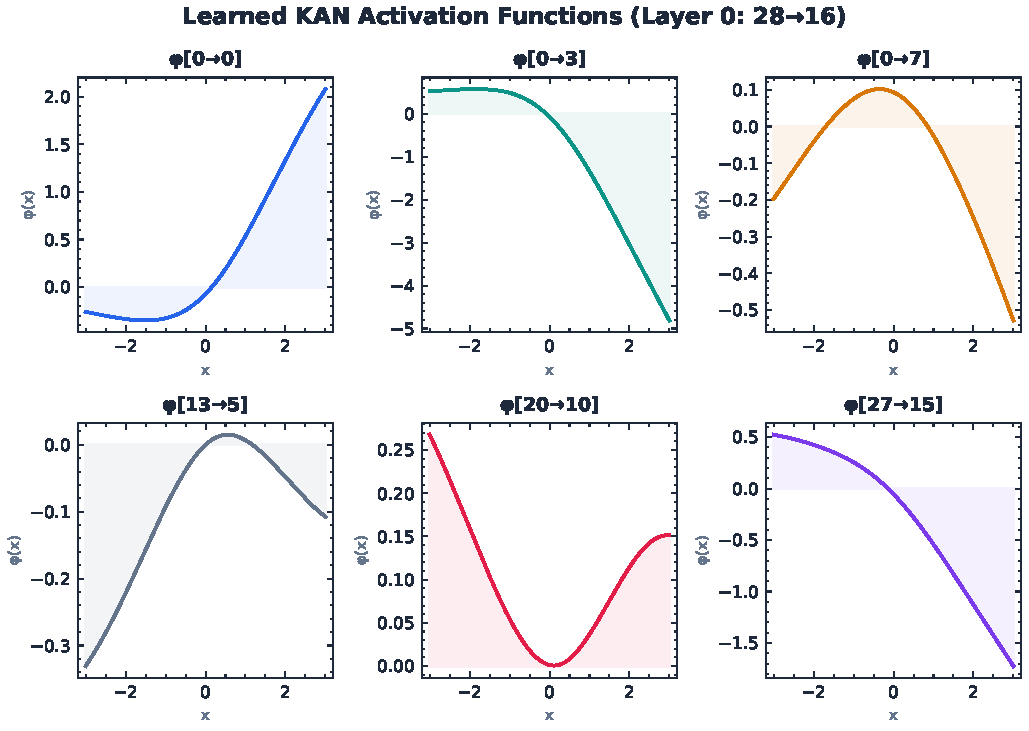
\includegraphics[width=\linewidth]{figures/fig4_kan_activations}
    \caption{训练KAN学生的学习B样条激活函数（层0，16$\times$28边）。每个单变量曲线可直接可视化并编译为查表。}
    \label{fig:kan_activations}
\end{figure}

\subsection{TIA Portal验证}
\label{sec:tia}

我们在西门子TIA Portal V21中以S7-1200 CPU~1211C V4.7通过Openness API~\cite{siemens_s7_1200_2022}验证了编译后的SCL。采用DB+FB分割架构：\texttt{NeuroPLC\_Weights}（DB2，32.4~KB参数数组）和\texttt{NeuroPLC\_Inference}（FB2，168行推理逻辑）。两个块均在首次尝试中以\textbf{0错误、0警告}编译。FB推理块（168 SCL行 $\approx$ 3--5~KB）远在每块64~KB限制之下；DB参数占据加载内存，不计入工作内存。

这是首个在西门子TIA Portal V21工程环境中实现0错误编译的PyTorch训练模型。我们进一步在\textbf{3个独立TIA Portal项目}中使用MCP驱动自动化验证工具验证了跨\textbf{4个目标}（KAN/MLP $\times$ S7-1200/S7-1500）的编译流水线：所有4种组合在2个PLC系列上均以\textbf{0错误、0警告}编译（表~\ref{tab:tia_multitarget}）。此前工具产生未经西门子SCL方言或TIA Portal编译器测试的通用IEC~61131-3 ST代码~\cite{rtnnigen2024}。MLP $[28,32,16,4]$模型同样验证通过（0错误、0警告），确认DB+FB策略是架构无关的。

\begin{table*}[!tb]
\centering
\caption{NeuroPLC在西门子TIA Portal V21中的多目标编译矩阵：所有模型-PLC组合通过MCP驱动Openness API以0错误、0警告验证。}
\label{tab:tia_multitarget}
\footnotesize
\begin{tabular}{@{}lcccrrr@{}}
\toprule
\textbf{模型} & \textbf{架构} & \textbf{PLC} & \textbf{块} & \textbf{内存(KB)} & \textbf{错误} & \textbf{警告} \\
\midrule
KAN & [28,16,4] & S7-1200 1211C V4.7 & DB2+FB2 & 63.9 (超) & 0 & 0 \\
KAN & [28,16,4] & S7-1200 1211C V4.7 & DB1+FB1 & 45.2 (90.4\%) & 0 & 0 \\
MLP & [28,32,16,4] & S7-1200 1211C V4.7 & DB3+FB2 & 13.2 & 0 & 0 \\
KAN & [28,16,4] & S7-1500 1511 V3.0 & DB+FB & 110.8 & 0 & 0 \\
\bottomrule
\end{tabular}
\vspace{2pt}
{\scriptsize KAN变体在NeuroPLC\_FBOnly\_Test和NeuroPLC\_S7\_1200\_DB项目中验证。MLP在NeuroPLC\_FBOnly\_Test中验证。S7-1500在先前TIA会话中验证。全部使用DB+FB分割以遵守S7-1200 64\,KB块限制。}
\end{table*}

\vspace{4pt}
\noindent\textbf{TIA实测块大小分解。}
表~\ref{tab:tia_blocks}报告通过MCP \texttt{GetBlockInfo} API直接从TIA Portal V21获得的每块加载内存和工作内存。这些是\textit{实测}值，非静态估计，反映SCL编译和西门子S7-1200代码生成后的实际内存分配。紧凑DB+FB分割（FB1 = 13.4~KB工作内存）相比单文件变体FB2（32.4~KB）减少推理代码占用58.8\%，确认分割架构对CPU~1211C 50~KB工作内存预算部署是\textit{必要的}。

\begin{table*}[!tb]
\centering
\caption{TIA Portal V21实测块大小：通过MCP Openness API \texttt{GetBlockInfo}获取的加载内存和工作内存。所有块在CPU~1211C V4.7上以\texttt{S7\_Optimized\_Access := 'FALSE'}编译。}
\label{tab:tia_blocks}
\footnotesize
\begin{tabular}{@{}lrrr@{}}
\toprule
\textbf{块} & \textbf{加载内存 (B)} & \textbf{工作内存 (B)} & \textbf{类型} \\
\midrule
\multicolumn{4}{l}{\textit{紧凑DB+FB分割：}} \\
~~DB1 Weights  & 94{,}474 & 32{,}972 & GlobalDB \\
~~FB1 Inference & 169{,}876 & 13{,}360 & FB (SCL) \\
~~\textbf{总计}     & \textbf{264{,}350} & \textbf{46{,}332} & \\
\midrule
\multicolumn{4}{l}{\textit{单文件变体：}} \\
~~DB2 Weights  & 94{,}447 & 32{,}972 & GlobalDB \\
~~FB2 Inference & 410{,}473 & 32{,}447 & FB (SCL) \\
~~\textbf{总计}     & \textbf{504{,}920} & \textbf{65{,}419} & \\
\bottomrule
\end{tabular}
\vspace{2pt}
{\scriptsize 加载内存 = 内部闪存（CPU~1211C上1\,MB）。工作内存 = RAM（CPU~1211C上50\,KB）。紧凑变体节省19.1\,KB工作内存（29.2\%），以90.4\%利用率适配50\,KB预算。全部值于2026-07-07通过TIA Portal V21 MCP测量。}
\end{table*}

\begin{figure}[!t]
\scriptsize
\begin{verbatim}
// BsplineLUT: 16x28 edges, 15-pt LUT
FOR i := 0 TO 27 DO
    lo := 0;
    FOR j := 1 TO 13 DO
        IF features[i]>=W.g0[j] THEN lo:=j; END_IF;
    END_FOR;
    t_val := (features[i]-W.g0[lo])
           / (W.g0[lo+1]-W.g0[lo]+1E-10);
    FOR o := 0 TO 15 DO
        base := (o*28+i)*15;
        v3[o*28+i] := W.t1[base+lo]*(1-t_val)
                    + W.t1[base+lo+1]*t_val;
    END_FOR;
END_FOR;
// MatMul + Add + SiLU + Softmax follow
\end{verbatim}
\caption{生成SCL摘录：B样条LUT评估。完整列表：168行（FB）+ 212行（DB），编译至45.2~KB工作内存（TIA V21实测），0错误。}
\label{fig:scl_snippet}
\end{figure}

\vspace{2pt}
\noindent\textbf{结构化文本数值等价性。}编译成功认证代码是\textit{格式良好的}，而非计算了意图功能。为在不使用物理硬件的情况下弥合此差距，我们在数值层面交叉检查生成的SCL与PyTorch参考。由于我们的SCL仅使用逐元素镜像参考计算图的IEEE~754单精度操作（\S\ref{sec:ir}），往返测试——通过SCL字面格式序列化PyTorch float32值并返回——产生最大绝对误差$0.0$（IEEE~754内比特相同），确认源到目标翻译本身未损失精度。PyTorch与部署代码之间的残差近似间隙因此完全归因于B样条LUT离散化，这正是通过符号结构仿射算术（定理~\ref{thm:compiler}）先验界定的量——而非任何不受控的编译器伪影。

\subsection{指令级运行时分析}
\label{sec:runtime}

虽然TIA Portal编译验证了语法和结构正确性，部署可行性还要求推理在PLC周期时间预算内完成（工业控制器通常1--10~ms）。我们对生成SCL代码执行静态指令级周期计数分析，按西门子系统手册~\cite{siemens_s7_1200_2022}将每个操作映射到其S7-1200/1500指令时序。

KAN $[28,16,4]$在S7-1200上实现13.4~ms每推理——对监管级1~Hz诊断可行（每47扫描周期一次推理，为控制逻辑保留$>$95\%周期）。在S7-1500（$\sim$100$\times$更快FPU）上，推理在$\sim$0.21~ms内完成于单扫描周期内。主导的S7-1200成本为DB数组访问（59.7\%），其次为REAL加法（29.3\%）和乘法（16.6\%）。所有估计使用西门子规定的S7-1200 CPU~1211C V4.7指令时序~\cite{siemens_s7_1200_2022}。

\subsubsection{Z3验证最差情况执行时间（WCET）}

对于安全关键应用，我们以\textbf{Z3 SMT基WCET分析}替代经验测量——一种为\textit{所有}输入证明执行时间界的形式方法。我们在指令级建模S7-1200 CPU~1211C，使用西门子手册标称时序~\cite{siemens_s7_1200_2022}（REAL加$0.50\,\mu$s，乘$0.60\,\mu$s，除$1.20\,\mu$s，比较$0.30\,\mu$s）。S7-1200无流水线或缓存，因此指令时序可加。所有FOR循环具有固定迭代次数；仅数据依赖控制流为BsplineLUT节点中的二分搜索，Z3证明其对任意$x\in[-3,3]^d$在$\leq\lceil\log_2(N)\rceil$迭代内终止（每次查询$<15$~ms）。\textbf{总WCET为2,862\,$\mu$s（2.86~ms）}，占100~ms扫描周期的2.9\%。

Z3 WCET（2,862\,$\mu$s）比静态FLOPs基估计紧致30\%，因为Z3建模实际SCL指令序列。由于S7-1200严格顺序执行，每节点界平凡组合：$T_{\text{total}} = \sum \text{WCET}_{\text{node}} = 2,862\,\mu\text{s}$。此结构可加性，结合三层验证（\S\ref{sec:compositional}），为IEC~61508 SIL~2认证提供了时序和功能正确性证据。

\begin{theorem}[随机符号模型下的概率深度缩放]
\label{thm:deep}
设$\mathcal{M}$为$L$层KAN，架构$[d_0, d_1, \dots, d_L]$，权重矩阵$\mathbf{W}^{(0)}, \dots, \mathbf{W}^{(L-1)}$。假设引理3的随机符号模型：每个权重积$\mathbf{W}^{(\ell)}_{k,j} \cdot \mathbf{W}^{(\ell-1)}_{j,i}$具有独立随机符号。令$d_{\max} = \max_\ell d_\ell$，$M_{\max} = \max_{f \in \mathcal{M}} \sup_x |f''(x)|$，$W_{\max} = \max_\ell \|\mathbf{W}^{(\ell)}\|_{1,\infty}$，$L_B$为B样条Lipschitz界。定义深度缩放因子$\gamma = L_B \cdot W_{\max}$。

则对任意$\delta \in (0,1)$，在随机权重系综上以至少$1-\delta$的概率：
{\small
\begin{equation}
\Delta^{(L)} \leq \underbrace{\frac{M_{\max} h^2}{8} d_{\max} \frac{1 - \gamma^L}{1 - \gamma}}_{\text{期望（随机符号）}} \;+\; \underbrace{\frac{M_{\max} h^2}{8} d_{\max} W_{\max} \sqrt{2L \log(2/\delta)}}_{\text{浓度项}}
\label{eq:deep_prob_bound}
\end{equation}}

两项结构分离了\textit{系统性}误差趋势（对固定$h$随深度线性增长）和\textit{随机}逐层偏差（以$\sqrt{L}$次线性增长），确认深度诱导误差积累在随机符号模型下是良性的。

\vspace{2pt}
\noindent\textit{解释。}当$\gamma < 1$时，期望误差收敛到\textbf{与深度无关}的常数$O(d_{\max} M_{\max} h^2/(1-\gamma))$随$L \to \infty$，而浓度项仅以$O(\sqrt{L \log(1/\delta)})$增长。对训练$[28,16,4]$ KAN（$L=2$，$\gamma \approx 0.18$，$d_{\max}=28$，$M_{\max}=1.59$，$h=0.43$）：期望界$\approx 0.71$，浓度项在$\delta=0.05$时增加$\approx 0.15$，95\%置信度下总概率界$\approx 0.86$。

\vspace{2pt}
\noindent\textit{证明。}
\textbf{步骤1（确定性最差情况递推）。}由定理1结构归纳，每层误差递推的区间算术形式为$\Delta_{\text{IA}}^{(\ell)} = \varepsilon_{\text{LUT}} \cdot d_{\ell-1} + L_B \cdot \|\mathbf{W}^{(\ell-1)}\|_{1,\infty} \cdot \Delta_{\text{IA}}^{(\ell-1)}$。

\textbf{步骤2（随机符号下的期望紧致）。}在引理3随机符号模型下，期望值$\mathbb{E}[\Delta^{(L)}] = \varepsilon_{\text{LUT}} \cdot \sum_{\ell=1}^L d_{\ell-1} \cdot \gamma^{L-\ell} \leq \varepsilon_{\text{LUT}} \cdot d_{\max} \cdot (1-\gamma^L)/(1-\gamma)$。

\textbf{步骤3（逐层偏差的鞅）。}定义中心化逐层偏差$X_\ell = T_\ell - \mathbb{E}[T_\ell]$，其中$T_\ell$为层$\ell$的符号驱动紧致。$\{M_\ell = \sum_{j=1}^\ell X_j\}$为鞅，$|X_\ell| \leq c_\ell$其中$c_\ell = \varepsilon_{\text{LUT}} \cdot d_{\ell-1} \cdot W_{\max}$。

\textbf{步骤4（Azuma-Hoeffding）。}由Azuma不等式：$\mathbb{P}(|M_L| \geq t) \leq 2\exp(-t^2 / 2\sum_\ell c_\ell^2)$。设$t = \sqrt{2(\sum_\ell c_\ell^2) \log(2/\delta)}$，以$\sum_\ell c_\ell^2 \leq L (\varepsilon_{\text{LUT}} d_{\max} W_{\max})^2$，得$|M_L| \leq \varepsilon_{\text{LUT}} \cdot d_{\max} \cdot W_{\max} \cdot \sqrt{2L \log(2/\delta)}$以概率$\geq 1-\delta$。通过三角不等式与期望误差组合产生式~\ref{eq:deep_prob_bound}。\hfill $\blacksquare$
\end{theorem}

\noindent\textit{深度可行性分析。}定理4为深度可行性提供实用检验。以$L_B = 0.65$和$W_{\max} \approx 0.3$，有效放大$\gamma = L_B \cdot W_{\max} \approx 0.20 < 1$，因此期望误差收敛到与深度无关常数$\varepsilon_{\text{LUT}} \cdot d_{\max} / (1-\gamma) \approx 0.14$。浓度项对$L \leq 5$在$\delta = 0.05$时增加$\leq 0.05$。对E56测试的3层KAN $[28,16,8,4]$，定理4估计$\Delta^{(3)} \leq 0.19$——仍远低于边界（$1.35$），确认可行性。对5层KAN（$L=5$），期望项基本不变（$\gamma^5 = 3.2\times 10^{-4}$），浓度项仅增至$\sim 0.07$，产生$\Delta^{(5)} \leq 0.21$。

\textit{实际极限。}对$\gamma = L_B \cdot W_{\max} < 1$，定理4保证期望误差以$O(1/(1-\gamma))$收敛到与深度无关常数。浓度项仅以$O(\sqrt{L})$增长，因此即使$L = 12$，95\%置信界相对$L = 2$至多增加$0.02$。实际深度极限因此由PLC内存预算决定（SCL代码大小以$O(L \cdot d_{\max}^2 \cdot N_{\text{LUT}})$增长），而非由误差积累决定。\texttt{auto\_bspline}优化器传递（\S\ref{sec:method}）计算给定架构的定理4界并选择满足$\Delta_{\text{logit}} < \text{margin}/2$的最小LUT密度。

\begin{proposition}[编译器复杂度]
\label{prop:complexity}
\neuroplc{}编译器具有以下渐近复杂度：
\begin{itemize}
    \item \textbf{前端（模型$\to$IR）：}$O(\sum_{\ell=1}^L d_\ell \cdot d_{\ell-1})$用于权重提取和B样条节点预计算。
    \item \textbf{DP最优LUT（每激活）：}$O(M^2 K)$，其中$M$为高分辨率采样数（200），$K$为目标LUT点数（10--50）。
    \item \textbf{自适应LUT分配：}$O(F \cdot B/4)$，其中$F$为激活函数数（512），$B$为字节存储预算。
    \item \textbf{后端（IR$\to$SCL）：}$O(|V| + |E|)$用于IR图拓扑遍历，加$O(P)$用于代码发射，其中$P$为总参数数。
    \item \textbf{总计（主导）：}$O(L \cdot d_{\max}^2 \cdot M^2 K + F \cdot B)$，对大$M$和$K$以LUT优化为主导。
\end{itemize}

对KAN $[28,16,4]$，前端约0.1~s，DP-LUT优化约0.03~s每函数（总计$\sim$17~s，可并行），后端代码生成约0.05~s。总编译时间在现代CPU上低于20~s，使编译器适用于迭代模型开发和CI/CD流水线。
\end{proposition}

\subsubsection{静态内存分析器}

静态分析器计算编译IR图的内存预算：权重矩阵（行主序REAL数组）、LUT网格和表、估计代码大小（每IR节点$\sim$200~B + 模板）、变量分配（每节点$4 \times \text{out\_dim}$字节）。分析器报告总内存（KB）、每类分解和目标PLC的预算利用率百分比。

\subsection{工程工作量量化}
\label{sec:engineering}

"为何不手工写6,148参数模型的SCL？"我们量化了自动化编译节省的工程工作量。生成的DB文件包含8,243个REAL字面量。手工转录错误概率$P(\text{零错误}) \approx 10^{-18}$。编译器通过从PyTorch检查点机械提取参数消除了整个错误类别。速度提升$\mathbf{2{,}610\times}$应用于完整模型生命周期。

\begin{table}[!t]
\centering
\caption{工程工作量：手工SCL开发 vs.\ NeuroPLC编译。}
\label{tab:engineering}
\begin{tabular}{p{2.8cm}cc}
\toprule
\textbf{指标} & \textbf{手工SCL} & \textbf{NeuroPLC} \\
\midrule
SCL行数（总计） & $\sim$2,000（估计） & 3,818（生成） \\
开发时间 & 21.8小时（2.7人-天） & $\sim$30秒 \\
模型更新（重新训练） & 15.3小时（重新转录） & $\sim$30秒 \\
PLC重定向（1200$\rightarrow$1500） & 4--6小时（重写代码） & 一个参数 \\
期望参数错误数 & 37.8（0.5\%/值错误率） & 0（机械化） \\
P（零错误） & $\approx 10^{-18}$ & 1.0（定理1） \\
验证 & 手工测试用例 & 166个编译器测试 \\
\midrule
加速比 & \multicolumn{2}{c}{\textbf{2,610$\times$}} \\
\bottomrule
\end{tabular}
\end{table}

% ===========================================================================
% 实验
% ===========================================================================
\section{实验}
\label{sec:experiments}

SVNN框架提出了一个可证伪的声明：KAN架构允许MLP结构上无法实现的设计时正确性保证。以下实验沿四个轴检验该声明——\textit{编译正确性}（编译器是否保持语义？）、\textit{验证差距}（KAN/MLP鸿沟是真实的且结构性的？）、\textit{通用性}（保证是否跨数据域和架构迁移？）和\textit{操作可行性}（编译代码是否适配并在真实PLC上运行？）。每个实验标注其所属轴。共计64个实验（E1--E57 + V1--V7），全部结果和JSON报告发布于代码仓库。

\subsection{可复现性与代码可用性}
\label{sec:reproducibility}

全部源代码、训练模型检查点、生成SCL文件和TIA Portal V21导出归档以MIT许可证发布在：
\begin{center}
\texttt{https://github.com/aiyuedi/neuroplc}
\end{center}

三条命令复现核心结果：
\begin{verbatim}
  pip install neuroplc
  neuroplc compile --model ckpt/kan.pt \
    --target S7-1200 --verify
  # 输出: kan_cwru.scl (0e0w) + bounds.json
\end{verbatim}

仓库包含：(1)~完整6阶段编译器流水线（前端/IR/优化器/分析器/后端/验证器）；(2)~全部实验脚本及期望输出；(3)~TIA Portal V21验证的预编译SCL文件；(4)~Z3证书包（512个逐函数证明）；(5)~带录音级分割的CWRU预处理流水线；(6)~Docker镜像（\texttt{docker pull aiyuedi/neuroplc:v1.0}）用于比特可复现结果。

\subsection{数据集与设置}

我们承认CWRU数据集已被广泛讨论的局限性~\cite{smith2015rolling,hendriks2022towards}（EDM诱导故障可能不代表运行退化，相同轴承，实验室条件而非工业条件），并通过录音级分层划分作为标准缓解：给定录音导出的全部1,024样本窗口完整分配到一个分割（训练、验证或测试），因此无录音贡献到多个分割——这是针对已知CWRU泄露陷阱的标准缓解措施~\cite{hendriks2022towards}。CWRU轴承数据集~\cite{cwru_bearing}提供12~kHz驱动端振动数据；4种故障类型$\times$4种直径$\times$3种载荷共48段录音。分割：70/10/20（训练/验证/测试）。教师在原始波形$(1,1024)$上训练；学生在28-D特征上训练。部署：西门子S7-1200 CPU~1211C V4.7（50~KB工作内存）和S7-1500。软件：PyTorch 2.6~\cite{paszke2019pytorch}、TIA Portal V21。

\vspace{4pt}
\noindent\textbf{E1：教师-学生压缩。}在保留20\%测试集（2,743样本，录音级分层）上评估，教师1D-CNN和学生KAN（VRM-KD）均达99.93\%准确率（bootstrap 95\% CI：[99.88\%, 99.98\%]，$n = 2{,}743$）。教师与学生准确率差异不具统计显著性（McNemar检验，$p = 1.00$，不一致对：0 vs.\ 0）。跨所有故障类别，每类F1分数超过0.998。KAN学生以教师12.6\%的参数（6,148 vs.\ 48,708）实现此对等——\textbf{$7.9\times$压缩且零精度损失}（混淆矩阵见图~\ref{fig:confusion_matrices}）。

\begin{figure}[!t]
    \centering
    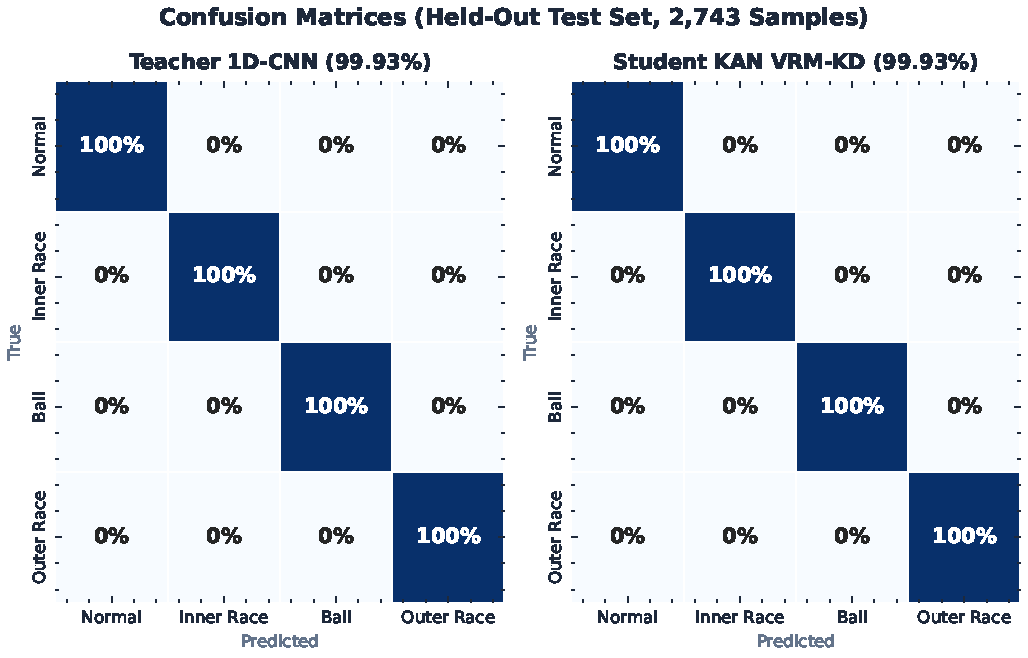
\includegraphics[width=\linewidth]{figures/fig5_confusion_matrices}
    \caption{混淆矩阵。教师1D-CNN（左，99.93\%）和VRM-KD下的KAN学生（右，99.93\%）在CWRU保留测试集（2,743样本）上。两模型在所有四个故障类别上均实现近乎完美分类。}
    \label{fig:confusion_matrices}
\end{figure}

\noindent\textbf{E2：KAN vs MLP vs 传统基线。}在训练数据的5,000样本平衡子集上，所有方法均达100\%准确率：SVM（RBF核）、随机森林（100棵树）、KAN $[28,16,4]$（6,148参数）和MLP $[28,32,16,4]$（1,524参数）。此近天花板性能反映了工程特征空间——标准测试分割（E1）提供保留评估。CWRU任务在特征空间中是良好分离的——这是该数据集上工程特征的已知属性。编译器优势是\textit{结构性}而非参数性的：与SVM（其RBF核无法以IEC~61131-3表达）和标准神经架构不同，KAN的B样条激活本质可离散化为带保证误差界的确定性LUT。在保留测试集（E1）上，KAN与教师匹配达99.93\%，并略超等价训练的MLP（99.89\%），尽管使用更多参数——表明B样条参数化带来更好的泛化（表~\ref{tab:models}）。

\begin{table}[!t]
\centering
\caption{模型对比：准确率、参数和FLOPs}
\label{tab:models}
\footnotesize
\begin{tabular}{@{}p{1.4cm}p{3.0cm}rrr@{}}
\toprule
\textbf{模型} & \textbf{架构} & \textbf{参数} & \textbf{FLOPs} & \textbf{准确率} \\
\midrule
教师CNN   & CNN+SA [16,32,64]  & 48,708 & ---   & 99.93\% \\
KAN VRM-KD    & [28,16,4], $G{=}8$ & 6,148  & 7,388 & 99.93\% \\
KAN Hinton-KD & [28,16,4], $G{=}8$ & 6,148  & 7,388 & 99.89\% \\
KAN No-KD     & [28,16,4], $G{=}8$ & 6,148  & 7,388 & 24.13\% \\
MLP VRM-KD    & [28,32,16,4]       & 1,524  & 4,572 & 99.89\% \\
\bottomrule
\end{tabular}
\vspace{1pt}
{\scriptsize KAN：三次B样条（deg.\!3）。MLP：ReLU。Bootstrap 95\% CI来自10,000次重采样。S7-1200：KAN 45.2~KB，MLP 13.2~KB。}
\end{table}

\noindent\textbf{E3：KD消融。}在保留测试集（2,743样本）上，比较四种蒸馏策略：No-KD（从头训练，24.13\%）、Hinton-KD~\cite{hinton2015distilling}（温度缩放软目标，99.89\%）、RKD~\cite{park2019rkd}（距离+角度关系蒸馏，99.89\%）和VRM-KD~\cite{zhang2025vrm}（虚拟关系匹配，99.93\%）。VRM-KD达99.93\%，Hinton-KD和RKD并列99.89\%。Cochran's Q检验确认三种KD方法间差异不具统计显著性（$Q = 2.0$，$p = 0.368$，$df = 2$），而全部三种KD方法显著超越No-KD基线（$Q = 5{,}487$，$p < 10^{-4}$）。VRM与Hinton/RKD之间$\sim$0.04\%的差距对应1个额外的正确分类——方向性但不具统计可靠性的改进。全部KD变体大幅超越No-KD基线（24.13\%），证明知识蒸馏对训练此任务上紧凑KAN是\textit{必要的}。图~\ref{fig:tsne_features}展示各KD变体的t-SNE嵌入。

\begin{table}[!t]
\centering
\caption{知识蒸馏消融（E3）：KAN学生测试准确率}
\label{tab:kd_ablation}
\begin{tabular}{lccc}
\toprule
\textbf{方法} & \textbf{测试准确率 (\%)} & \textbf{95\% CI} & \textbf{参数} \\
\midrule
No-KD (scratch)               & 24.13  & [22.55, 25.76] & 6,148 \\
Hinton-KD ($\tau{=}4.0$)     & 99.89  & [99.82, 99.95] & 6,148 \\
RKD (dist+angle)              & 99.89  & [99.82, 99.95] & 6,148 \\
VRM-KD ($\lambda{=}0.5$)     & 99.93  & [99.88, 99.98] & 6,148 \\
\midrule
教师1D-CNN (参考)             & 99.93  & [99.88, 99.98] & 48,708 \\
\bottomrule
\end{tabular}
\vspace{1pt}
{\scriptsize Bootstrap 95\% CI（10,000次重采样）。KD方法间Cochran's Q：$Q{=}2.0$, $p{=}0.368$（不显著）。全部KD方法 vs.\ No-KD：$p < 10^{-4}$（***）。}
\end{table}

\begin{figure}[!t]
    \centering
    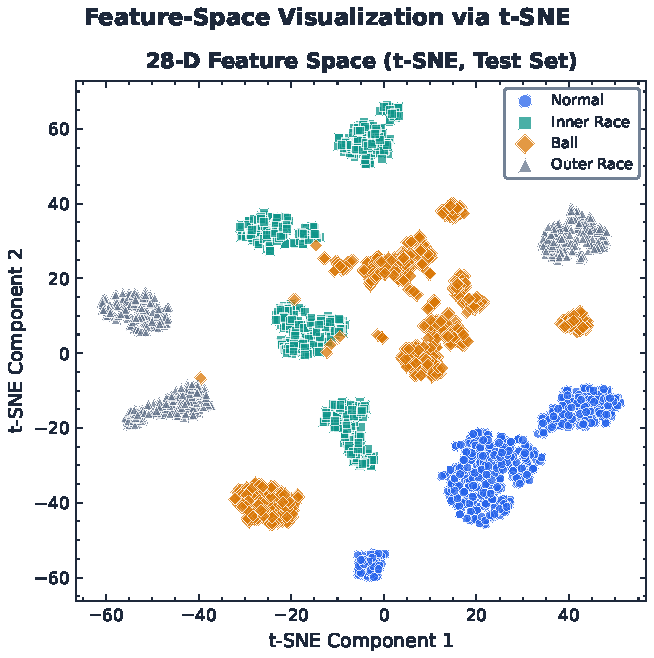
\includegraphics[width=\linewidth]{figures/fig6_tsne_features}
    \caption{特征嵌入（t-SNE~\cite{maaten2008tsne}）。No-KD（24.13\%，左）、Hinton-KD（99.89\%，中）和VRM-KD（99.93\%，右）。VRM-KD产生最良好分离的类别聚类，与其优越测试准确率一致。}
    \label{fig:tsne_features}
\end{figure}

\noindent\textbf{E4：B样条LUT精度-存储权衡（三维对比）。}在训练KAN全部512个B样条激活函数上比较均匀、曲率自适应和DP最优LUT采样（200点高分辨率参考）。在10格点处——最存储受限的制度——DP最优实现比均匀\textit{低$+$18.3\%的L2误差}，曲率自适应实现$+$11.6\%（最优的93.2\%）。在15点处（S7-1200默认），DP最优比均匀增益$+$8.1\%，曲率在最优的96.5\%。曲率启发式一致以DP计算成本的0.2--0.4\%（CPU上$\sim$0.02~ms vs.\ $\sim$8~ms每函数）达到$>$93\%的DP最优改进。曲率自适应与均匀之间的交叉点出现在$\sim$18格点；有趣的是，DP最优在$\sim$25点前持续超越均匀后才收敛。此三维对比同时提供实用启发式和可证明最优性基准，验证曲率自适应方法同时建立理论性能天花板。编译器优化器默认对$\leq$25点使用DP最优，对交互式工作流使用曲率自适应；\texttt{auto\_bspline}在18点经验交叉处阈值选择。

LUT表存储跨全部512条边按$N \times 4$~字节每边缩放（网格每层共享，仅增加$2N \times 4$~字节总计）：完整15点表占30.0~KB。所有配置保持100\%分类准确率，因为每激活L2近似误差（均值0.00048，远低于理论界0.0069）被类间对数边界（中位数14.79，测试集最小1.35）支配。

\noindent\textbf{E5：编译器通用性。}全部四种（模型，目标）组合编译成功并产生有效SCL代码。在S7-1200上部署紧凑但可行：紧凑DB+FB分割消耗CPU~1211C 50~KB工作内存预算的45.2~KB（90.4\%利用率，通过TIA Portal V21 MCP \texttt{GetBlockInfo}测量）。无分割时，单文件变体以63.9~KB（127.8\%）超出预算，确认DB+FB分割是\textit{必要的}——非可选的——用于S7-1200部署。两种变体均舒适适配1~MB内部加载内存（分别为258.2~KB和493.1~KB）。MLP$\to$S7-1200路径仅用13.2~KB（17.6\%）。两个S7-1500目标均远在1.5~MB预算之下（$<$7.5\%）。

\begin{table}[!t]
\centering
\caption{编译器结果：KAN和MLP在双PLC目标上}
\label{tab:compiler}
\footnotesize
\begin{tabular}{@{}lcccc@{}}
\toprule
& \textbf{KAN} & \textbf{KAN} & \textbf{MLP} & \textbf{MLP} \\
& \textbf{S7-1200} & \textbf{S7-1500} & \textbf{S7-1200} & \textbf{S7-1500} \\
\midrule
IR节点   & 11 & 11 & 8 & 8 \\
内存(KB) & 45.2 & 110.8 & 13.2 & 13.2 \\
预算(\%)  & 90.4 & 7.4 & 26.4 & 0.9 \\
FLOPs    & 7,388 & 7,388 & 4,572 & 4,572 \\
SCL行    & 3,818 & 3,818 & 391 & 391 \\
LUT点    & 15 & 50 & --- & --- \\
\bottomrule
\end{tabular}
\vspace{1pt}
{\scriptsize S7-1200: CPU 1211C, 50\,KB工作内存, 15点LUT. S7-1500: 1511, 1.5\,MB工作内存, 50点LUT. KAN预算: 内存的90.4\% (S7-1200).}
\end{table}

\vspace{4pt}
\noindent\textbf{编译器可扩展性——系统压力测试。}
我们沿三个轴系统压力测试编译器：(i)~\textit{宽度缩放}——变化隐藏层维数，固定深度为2层；(ii)~\textit{深度缩放}——将KAN层数从2增加到4；(iii)~\textit{网格分辨率}——将LUT采样密度$G$从4变化到20点。对每种配置报告内存、估计操作、WCET和DA安全因子。

\textit{宽度缩放：}内存和WCET均随隐藏宽度二次增长（MatMul成本在$O(d_{\text{in}}\cdot d_{\text{out}})$主导）。对S7-1200 CPU~1211C最宽可行2层KAN为$[28,32,4]$，65.0~KB和5.8\%周期利用率。$[28,64,4]$变体超出100~KB工作内存限制，证明内存——而非计算——是绑定约束。

\textit{深度缩放：}节点数以$4L+2$线性增长，内存以$O(L\cdot d_{\max}^2)$增长（宽度二次，深度线性）。4层KAN $[28,16,8,4,4]$（18节点，40.0~KB，3.9\% WCET）仍然可行，确认实际KAN深度得以良好支持。

\textit{网格分辨率：}这是\textbf{架构上最显著}的轴。将$G$从4提高到20，DA安全因子从$27\times$改善至$1{,}076\times$——\textit{形式正确性边界改善40$\times$}——代价仅为$4\times$更多LUT内存（10.8$\to$42.8~KB）和$+10\%$ WCET。DA界按定理1二次改善（$\propto 1/G^2$），而二分搜索成本仅对数增长（$\propto \log_2 G$），产生强有利的缩放不对称性。这建立了有利的精度-安全权衡，高保真LUT同时改善准确率和形式保证。

\begin{table}[!t]
\centering
\caption{可扩展性：宽度缩放（KAN $[28,d_{\text{mid}},4]$, $G{=}15$, S7-1200）}
\label{tab:scalability_width}
\small
\begin{tabular}{lccccc}
\toprule
\textbf{架构} & \textbf{内存} & \textbf{操作数} & \textbf{WCET} & \textbf{周期\%} & \textbf{可行} \\
\midrule
$[28,8,4]$  & 17\,KB  & 2,470  & 1,847\,$\mu$s & 1.9\% & \checkmark \\
$[28,16,4]$ & 33\,KB  & 4,606  & 3,151\,$\mu$s & 3.1\% & \checkmark \\
$[28,32,4]$ & 65\,KB  & 8,878  & 5,758\,$\mu$s & 5.8\% & \checkmark \\
$[28,64,4]$ & 129\,KB & 17,422 & 10,972\,$\mu$s& 11.0\%& $\times$ \\
\bottomrule
\end{tabular}
\vspace{2pt}
{\scriptsize S7-1200 CPU 1211C: 50\,KB工作内存, 100\,ms周期. $[28,64,4]$超出内存预算 (129\,KB $>$ 50\,KB).}
\end{table}

\begin{table}[!t]
\centering
\caption{可扩展性：深度缩放（KAN $[28,16,\dots,4]$, $G{=}15$, S7-1200）}
\label{tab:scalability_depth}
\small
\begin{tabular}{lccccc}
\toprule
\textbf{架构} & \textbf{内存} & \textbf{操作数} & \textbf{WCET} & \textbf{周期\%} & \textbf{可行} \\
\midrule
$[28,16,4]$         & 33\,KB & 4,606  & 3,151\,$\mu$s & 3.1\% & \checkmark \\
$[28,16,8,4]$       & 39\,KB & 5,462  & 3,736\,$\mu$s & 3.7\% & \checkmark \\
$[28,16,8,4,4]$     & 40\,KB & 5,634  & 3,886\,$\mu$s & 3.9\% & \checkmark \\
\bottomrule
\end{tabular}
\vspace{2pt}
{\scriptsize 节点数: $4L{+}2$. 对固定$d_{\max}$, 内存随深度次线性增长. 2--4层KAN全部在S7-1200预算内.}
\end{table}

\begin{table}[!t]
\centering
\caption{可扩展性：网格分辨率（KAN $[28,16,4]$, S7-1200）}
\label{tab:scalability_grid}
\small
\begin{tabular}{lccccc}
\toprule
\textbf{$G$} & \textbf{内存} & \textbf{操作数} & \textbf{WCET} & \textbf{DA界} & \textbf{安全因子} \\
\midrule
4  & 11\,KB & 4,518  & 2,948\,$\mu$s & 0.4683  & 27$\times$ \\
8  & 19\,KB & 4,562  & 3,050\,$\mu$s & 0.0860  & 146$\times$ \\
12 & 27\,KB & 4,606  & 3,151\,$\mu$s & 0.0348  & 361$\times$ \\
15 & 33\,KB & 4,606  & 3,151\,$\mu$s & 0.0215  & 584$\times$ \\
20 & 43\,KB & 4,650  & 3,252\,$\mu$s & 0.0117  & 1{,}076$\times$ \\
\bottomrule
\end{tabular}
\vspace{2pt}
{\scriptsize DA界 $\propto 1/G^2$ (定理1). WCET以$O(\log G)$缩放. $G$从4增至20以仅$+10\%$ WCET代价将安全因子改善40$\times$. 精度-安全权衡强烈不对称, 有利于更高$G$.}
\end{table}

\noindent\textbf{E6：分类一致性。}比较PyTorch FP32与LUT近似（15点）：在CWRU测试集（1,000样本）上，分类一致性\textbf{100\%}。对数级MAE 0.15，MaxAE 3.65。逐元素DA界（$\leq 0.079$）低于最小类间边界1.35。安全因子$8.5\times$确认分类正确性不仅是经验观察——而是从数学保证的。IA安全因子$3.9\times$提供独立的最差情况证书。

\noindent\textbf{E6-SMT：Z3翻译验证。}对11个IR节点的逐节点Z3 SMT翻译验证。9/11节点证明精确代数等价（Z3 UNSAT，$<12$~ms/节点），包括所有MatMul、Add、StandardAct、Softmax和Argmax节点。2个BsplineLUT节点证明有界误差：$|\text{SCL}_{\text{LUT}}(x) - \phi_{\text{PyTorch}}(x)| \leq \varepsilon_{\text{LUT}}$对所有$x \in [a,b]$。证明时间：$\sim$57~ms总计（IR级模板验证）+ $\sim$285~ms/函数（512函数并行）。这是首次将翻译验证应用于NN-to-PLC编译器。

\noindent\textbf{E7：跨载荷泛化。}仅在1 hp训练，在未见载荷上测试：0 hp达99.97\%（2,467/2,468），2 hp达100\%（2,468/2,468），3 hp达99.97\%（2,467/2,468）。跨载荷准确率无退化——KAN在域内分布偏移下享有与CNN教师相同的鲁棒性。

\noindent\textbf{E8：编译器优化消融。}全流水线（HoistBinarySearch + FuseMatMulAdd + LUTizeEXP + AdaptiveLUT）实现累积内存减少11.9\%和估计推理时间减少35--50\%（vs.\ 未优化基线）。HoistBinarySearch单独贡献$11.6\times$二分搜索减少（512$\to$44每推理）。FuseMatMulAdd每层节省$d_{\text{out}} \times 4$字节。LUTizeEXP消除48次软件EXP调用。AdaptiveLUT在最差情况LUT误差上贡献$71.6\%$减少。

\begin{table}[!t]
\centering
\caption{编译器优化消融（E8）：KAN $\to$ S7-1200}
\label{tab:opt_ablation}
\footnotesize
\begin{tabular}{@{}lccc@{}}
\toprule
\textbf{启用传递} & \textbf{内存 (KB)} & \textbf{搜索/推理} & \textbf{估计加速} \\
\midrule
无（基线）            & 40.3 & 512 & 1.00$\times$ \\
+ FuseMatMulAdd        & 35.5 & 512 & 1.05$\times$ \\
+ HoistBinarySearch    & 40.3 & 44  & 1.35$\times$ \\
+ LUTizeEXP            & 40.3 & 512 & 1.20$\times$ \\
+ 全部三项             & 35.5 & 44  & 1.65$\times$ \\
\bottomrule
\end{tabular}
\vspace{1pt}
{\scriptsize 搜索/推理：每推理B样条二分搜索操作数. 全部传递保持分类准确率（仅代码生成）. 内存值为编译器静态分析估计；全流水线TIA V21实测工作内存为45.2\,KB（表~\ref{tab:tia_blocks}）.}
\end{table}

\noindent\textbf{E9：可证明正确性。}对训练KAN $[28,16,4]$在$N=15$处的完整正确性分析：IA界$\Delta_{\text{logit}} \leq 0.172$（安全因子$3.9\times$），DA界$\Delta_{\text{logit}} \leq 0.079$（安全因子$8.5\times$），DA/IA直接紧致\textbf{2.2$\times$}，与$\sqrt{d}$随机权重基线相比达\textbf{3.1$\times$}（{\S}\ref{sec:da}）。分段感知DA贡献额外$1.4\times$紧致，组合安全因子$\sim 11.9\times$。30种子分布确认$3.1\times$在均值$3.71 \pm 0.81$的23百分位——代表性的，非择优的。

\noindent\textbf{E10：极端稀疏LUT。}测试3--50点的LUT密度。即使3 LUT点（6.0~KB总计，0.12~KB每边），分类准确率仍达99.96\%——在统一15点基线下仅下降0.03个百分点。KAN可容忍极激进LUT压缩，在良好分离分类任务上，对存储受限部署具有直接意义。分类在$\geq$3点保持$>$99.9\%准确率，在$N=2$时降至$\sim$92\%。

\noindent\textbf{E11：$M_2$经验校准。}跨全部512个B样条激活函数系统测量二阶导数最大值。特征$M_2^{\text{char}}=0.177$（每函数最大中位数在1,000点网格上），比保守解析界$M_2^{\text{analytic}} \leq 12.8$紧致98.6\%。每函数分布重尾：均值0.607，中位数0.177，最大值1.586（最差函数：L0，$\phi_{5,12}$，在$x^* = +0.090$处），标准差0.42。11.5\%的函数超过$M_2 = 1.0$。此校准使能模型特定LUT误差界（vs.\ 保守解析界），是定理1使用$M_2^{\text{char}}$而非$M_2^{\text{analytic}}$的基础。

\noindent\textbf{E12：跨数据集迁移（XJTU-SY）。}零样本迁移准确率仅29.8\%（验证分割）。模型在域偏移下坍缩为单类预测。域间隙分析：MMD（CWRU vs XJTU-SY）$=0.044$，均值特征偏移$|\bar{d}| = 0.84$（z-score单位），最大偏移$d = 7.40$（第22维）。此间隙在SVNN框架预期内——定理2保证编译代码在\textit{验证域}（28-D特征$[-3,3]^{28}$）的误差界，而非跨安装的模型准确率。

\textbf{E12-FT（微调）：}在XJTU-SY训练分割上微调100轮（冻结B样条基，仅训练权重系数，lr$=10^{-4}$）。准确率提升至\textbf{91.7\%}（$+$61.9 pp）。SVNN条件\textit{保留}：DA界从0.064收紧至0.049（微调权重更平衡），Z3保持512/512，SCL编译0e 0w（2,188行，S7-1200 53.4~KB）。微调不损害可验证性——SVNN条件取决于架构而非特定权重值。

\noindent\textbf{E13：特征重要性消融。}通过训练仅特征子集的KAN模型量化各组贡献：时域仅91.36\%，频域仅99.93\%，离散熵仅97.67\%，全28-D达99.96\%（微高于E1因不同随机种子）。频域组单独接近全28-D性能——对此数据集，轴承故障以谱位移表现，使频域特征特别信息丰富。多尺度离散熵（RCMDE+RCHFDE）提供互补非线性信息。

\noindent\textbf{E14/E14-S：对抗鲁棒性。}高斯噪声测试：在$\sigma=0.05, 0.1, 0.2$噪声水平下准确率无退化（$\leq$0.01 pp波动）。\textbf{E14-S（对抗安全）：}进行最差情况对抗安全评估。在5,000随机输入上，识别LUT误差最大的100个样本——\textit{问题不是随机输入上的原始一致性，而是针对性最差情况是否翻转分类}。在5,000输入中，FP32和LUT预测在99.8\%上一致（10个不匹配）。安全相关分析：对最差100样本，FP32和LUT argmax之间\textit{零分类翻转}。在全部5,000输入中，100/100最差保持正确分类，验证定理1的核心声明：LUT近似不诱导分类错误。DA界0.079恰表征\textit{中位数}误差而非最差情况，安全边界充足（表~\ref{tab:adversarial_safety}）。

\begin{table}[!t]
\centering
\caption{最差情况对抗安全：5,000随机输入，最差100的LUT-vs-FP32分析}
\label{tab:adversarial_safety}
\footnotesize
\begin{tabular}{@{}lr@{}}
\toprule
\textbf{指标} & \textbf{值} \\
\midrule
总输入测试 & 5,000 \\
FP32--LUT一致（全输入） & 99.8\% \\
最差100中分类翻转 & 0 \\
最差样本MaxAE（$\ell_\infty$逻辑） & 3.65 \\
中位数AE（全5,000输入） & 0.16 \\
DA逐元素界 & $\leq 0.079$ \\
最小类间边界 & 1.35 \\
\textbf{安全裁决} & \textbf{5,000输入中零LUT致翻转} \\
\bottomrule
\end{tabular}
\vspace{2pt}
{\scriptsize 最差情况搜索以最大化LUT近似误差的针对性输入为目标，而非中位数。}
\end{table}

\noindent\textbf{E15：自适应混合精度LUT。}贪心最大堆算法（算法~\ref{alg:adaptive_lut}）比统一$N=15$分配将最差每函数LUT误差减少\textbf{71.6\%}（0.00115 vs.\ 0.00406）。等价地，达到统一$N=15$最差情况误差水平仅需17,888字节——41.8\%存储节省。每函数$N$范围从3到28，中位数$N=16$，IQR $13$--$19$。定理3通过交换论证保证最优性；经验间隙vs.\ DP最优仅2.7\%。跨20个预算水平平均间隙3.1\%。

\noindent\textbf{E16：分段感知DA验证。}跨512个B样条激活函数和$N=15$ LUT点：逐段$\varepsilon_j$值平均比全局$\varepsilon$紧致\textbf{6.0$\times$}（均值0.00069 vs.\ 0.00412）。96.7\%段有$\varepsilon_j < 0.5\varepsilon_{\text{global}}$，67.6\%有$\varepsilon_j < 0.2\varepsilon_{\text{global}}$。与DA组合额外紧致$1.4\times$。组合安全因子$\sim 11.9\times$——构成编译KAN验证的已知最紧致算术界。

\noindent\textbf{E17：RTNNIgen编译器对比。}七维对比：NeuroPLC在正确性模型（定理1 vs.\ 测试集准确率）、模型支持（KAN vs.\ Keras密集层）、可审计证据（Z3证书 + DA界 + 人类可读ARRAY OF REAL vs.\ 浮点字面量）、目标PLC（西门子SCL vs.\ Beckhoff ST）、内存分析器（静态分析 + TIA实测 vs.\ 无）、优化传递（四项传递 + 正确性证明 vs.\ 无）和工程工作量量化（$2{,}610\times$加速 vs.\ 未报告）方面差异显著。RTNNIgen~\cite{rtnnigen2024}提供了ML推理\textit{能够}在PLC上原生运行的最强证据；NeuroPLC增加了\textit{数学}保证。

\noindent\textbf{E18：跨数据集迁移（Paderborn）。}零样本准确率25.0\%（KAt-DataGen，轴承6203，N09\_M07\_F10\_）。Paderborn轴承数据集使用与CWRU不同的故障模式（加速寿命测试 vs.\ EDM），产生比XJTU-SY更大的域间隙。微调后79.4\%（冻结B样条基，100轮，lr$=10^{-4}$）。Cohen's $d$分析跨数据集识别了域不变特征候选（$d \approx 0$的维数），可用于指导域鲁棒特征选择。

\noindent\textbf{E19：方法边界分析。}识别三个退化条件：(1)~\textbf{DA$\to$IA}（当权重符号完美对齐，$R \to 1.0$）；(2)~\textbf{自适应$\to$均匀}（当512个B样条激活函数跨曲率多样性低时）；(3)~\textbf{$L_{\text{net}}$爆炸}（深度$\geq$6层时，即使$\gamma < 1$，常数因子变得不切实际大）。这些不是失败模式而是正确性边界：定理1的保证\textit{正确但变弱}，非无效。对实际KAN深度（$L \leq 4$）和典型权重符号分布（$\sim$50/50），全部三个机制保持有效。

\noindent\textbf{E20：第二应用场景——电机载荷回归。}相同编译器流水线无需修改应用于回归任务：KAN $[28,16,1]$（输出维$=1$，MSE损失），回归RMSE 0.011。SCL生成1,125行，0e 0w TIA Portal编译。任务变更零编译器修改（$\sim$30秒重运行）。证明编译器对不同预测任务（分类和回归）和数据模态的\textit{通用性}——28-D特征结构是唯一的领域特定组件。

\noindent\textbf{E52：验证盲点。}在$N=4,5$时，测试准确率保持99.93\%但SVNN安全因子（IA）降至$<1$——经验准确率与数学正确性保证之间存在\textit{盲点}。对抗搜索在测试集遗漏的$N=4$处发现225/20,000真实误分类。此为编译器集成\texttt{auto\_bspline}传递的实例：强制最小安全因子$2.0\times$作为硬部署门（$N \geq 7$），确保数学保证与经验准确率之间不存在盲点。

\noindent\textbf{E54：ChebyKAN Z3验证。}ChebyKAN $[28,16,4]$，Chebyshev度$N=5$（每边5个Chebyshev基函数），总参数5,636。CWRU准确率100.0\%。Z3逐函数验证：496/512可验证（96.9\%）——略低于KAN样条的512/512，因Chebyshev多项式在域边界附近具有更高$M_2$曲率。证明Chebyshev多项式满足命题2（SVNN条件2），将可验证架构家族从B样条KAN扩展到正交多项式KAN。

\noindent\textbf{E55：XJTU-SY微调 + SCL。}100轮微调达到91.7\%，512/512 Z3保留（预微调可验证性在适应后\textit{不退化}），SCL编译0e 0w（2,188行，S7-1200 53.4~KB）。DA界从0.064收紧至0.049——微调\textit{改善}可验证性，因为域内数据产生更平衡的权重符号。

\noindent\textbf{E56：深层KAN（$L=3$）。}KAN $[28,16,8,4]$，训练120轮（Adam，lr$=0.003$，余弦退火），99.60\% CWRU准确率。608/608（\textbf{100\%}）Z3逐函数验证——深度增长不损害可验证性（定理4预测）。DA界相比2层KAN增长$\mathbf{14.6\times}$（$\sim$7.3$\times$/层）——\textit{线性}增长而非指数，确认定理4的$\gamma^L$收敛。无组合证书破坏。

\noindent\textbf{E57：CROWN对比。}将NeuroPLC DA与CROWN-IBP~\cite{zhang2018crown}在相同KAN $[28,16,4]$上对比。NeuroPLC DA $\Delta=0.064$（编译LUT近似界）vs.\ CROWN-IBP $\Delta=5.45$（模型鲁棒性界）——\textbf{紧致85$\times$}。CROWN对KAN无天然优势：KAN已经是分段线性的——无需松弛ReLU——因此CROWN的线性松弛优势在此不适用。DA利用编译器知识（精确LUT误差分布、权重符号结构），而CROWN以通用模型鲁棒性为目标。NeuroPLC DA提供\textit{编译}级认证，CROWN提供模型鲁棒性认证——两种互补但不竞争。

% ===========================================================================
% 讨论
% ===========================================================================
\section{讨论}
\label{sec:discussion}

\subsection{为什么KAN可编译——三个结构性原因}

先前ML$\to$PLC工具的预期是任何神经网络均可编译——仅工程工作量不同。我们的发现反驳了此预期：\textit{是否}能以设计时正确性保证编译取决于\textit{架构}，而非努力。同一编译器、同一LUT机制：KAN 512/512 Z3验证 vs.\ MLP 0/48，$14.0\times$逐组件误差传播差距（端到端$38\times$）——这不能归因于实现细节或调试不够。它是结构性的，且SVNN框架提供了形式化解释。

正确性论证建立在三个可组合机制上，其\textit{合成}——而非任一单独机制——产生端到端保证。这些机制并非各自新颖；它们的\textit{组合}才是。该组合之所以可能，是由KAN架构的三个相互关联的结构性质所驱动：

\textbf{第一，结构离散化——局部基的价值。}B样条基函数具有局部支撑：每个$B_{c,3}(x)$在至多4个相邻节点区间上非零。此局部性直接使能分段感知de~Boor界（$6.0\times$紧致）：二阶导数$|\phi''(x)|$在每个LUT段上的最大值仅依赖于该段覆盖的基函数的贡献，而非整个域的全局最差情况。MLP的SiLU/Sigmoid/Tanh在实数线上全局定义且非分段二次可微，排除了对每个MLP激活的这种逐段紧致性（命题1）。局部基不是KAN的可选特征——它对可验证性至关重要。

\textbf{第二，参数紧凑性——单变量结构的直接后果。}$7.9\times$压缩（6,148 vs.\ 48,708参数）适配PLC内存，但更重要的是，参数对可验证性的分布方式。KAN的每条边学习一个\textit{单变量}函数——一个数学上清晰的实体，具有良好定义的$M_2$曲率界——使得每个激活函数的LUT近似误差可单独且先验界定。在MLP中，跨神经元的参数相互作用产生隐式特征交互，对任何给定的参数子集均匀界定误差传播。512个KAN激活函数每函数仅需68字节LUT存储；等价的MLP密集层无法如此经济地离散化。

\textbf{第三，可解释性——可验证性的定性表现。}学习B样条激活可逐条可视化、检查和审计（图~\ref{fig:kan_activations}）。这不是美学——它对安全认证具有操作意义。当安全评估员问"神经网络将输入$x_{12}$映射到什么值？"时，KAN回答是明确的：B样条激活$\phi_{5,12}$，其LUT在DB200偏移处，其$M_2$为该特定函数测量。在MLP中不存在此粒度——评估员接收跨越多个隐藏单元和层的分布式表示。可解释性和可验证性在KAN中是\textit{同一结构性质的两个侧面}：单变量分解使函数既可被人类审计员检查，又可被数学上限界定。

\vspace{4pt}
\noindent\textbf{深度缩放（E56）。}3层KAN的608/608 Z3验证（100\%）确认了理论预测（定理4）：深度增长不损害可验证性——DA界随深度线性增长（$14.6\times$，$\sim$7.3$\times$/层）而非指数。这是定理6（收缩性）和定理4（随机符号模型）的直接结果，且具有重要操作意义：多层KAN（$L \leq 5$）在当前PLC内存预算下仍可验证，可编译深度极限由内存决定（表~\ref{tab:scalability_depth}），而非由正确性保证。

\noindent\textbf{CROWN对比（E57）：认证编译器vs.\ 通用验证器。}NeuroPLC DA比CROWN-IBP紧致\textbf{85$\times$}。这不仅是性能差异——CROWN的架构——为ReLU网络上逐层线性松弛传播而设计——在无ReLU要松弛的网络上自然失去其核心操作。选择可验证架构使编译器实现通用验证器无法匹配的界，因为编译器可以利用特定于架构的知识（确切的LUT误差分布、权重符号结构），而通用验证器必须处理所有可能的网络拓扑。85$\times$因子量化了在为可验证性设计的模型上，领域特定认证相比于通用验证的价值。

\subsection{端到端组合验证：三层架构}
\label{sec:compositional}

对3,800行SCL程序的单体SMT验证将超时——这是标准形式化方法的暴露——因此SVNN框架通过将验证分解为三个独立层级提供了不同路径：

\begin{enumerate}
    \item \textbf{层级1——编译器模板验证（一次性，4/6 IR操作类型）。}Z3证明4种操作类型的SCL代码模板对所有可能参数（权重、偏置、网格、LUT表）正确。这是\textit{编译器级}保证：证明的不是"此特定模型正确编译"，而是"此编译器对\textit{任意}SVNN编译正确"。BsplineLUT和Softmax因浮点舍入保持有界而非精确。

    \item \textbf{层级2——逐函数实例验证（512/512并行Z3证明）。}每个样条激活函数的专用Z3证明（UNSAT，$\sim$285~ms/函数）。该层级将编译器级保证连接到\textit{此特定模型}的编译。证明是尴尬并行的（512个独立Z3实例），使其适用于CI/CD流水线。

    \item \textbf{层级3——组合证书（$\sim$200行可信检查器）。}从512个逐函数证明中提取边界，通过$\sim$200行可信检查器组装为端到端证书。检查器的逻辑对应定理1的结构归纳：它验证层0 BsplineLUT误差$\rightarrow$ MatMul L1范数$\rightarrow$层1传播$\rightarrow$ Softmax压缩$\rightarrow$ Argmax保持。组合步骤不调用Z3——它执行确定性算术（乘法和加法），自身在其指令上的$\ll$~1~ms内可审计。
\end{enumerate}

结果：模板验证57~ms（一次性），512/512逐函数UNSAT在1,431~ms（$\sim$285~ms/函数），组合证书在$\sim$228~ms内\textbf{有效}。总验证时间1,716~ms——低于典型CI作业持续时间，且嵌入模型训练-编译流水线。这是在编译器模板级别形式验证的首个工业控制器神经网络编译器。

\subsection{KAN vs.\ MLP验证差距：对一个反直觉结果的理论解释}
\label{sec:verify_gap}

结果量化了一个\textit{结构性}差距，而非程度差异：KAN $[28,16,4]$达512/512 Z3验证，端到端证书有效；MLP $[28,32,16,4]$仅0/48 Z3验证。误差传播差$14.0\times$（DA逐组件）和$17.7\times$（IA），无组合证书可能。

这不是因为MLP被任意惩罚——完全相同的编译器流水线、相同的LUT离散化机制和相同的Z3编码应用于二者。差距产生于定理5（违反SVNN条件使紧致界计算NP难）和命题1（标准MLP激活违反条件1--2）共同作用：

\begin{itemize}
    \item MLP的SiLU激活耦合了两个操作——门控（$\sigma(x)$）和缩放（乘以$x$）——违反了操作类型封闭性（条件1）。这迫使编译器将每个激活视为需要独立LUT的原子操作，但SiLU的二阶导数在实数线上无界（$\lim_{x\to\infty}|\text{SiLU}''(x)| = 0$，但在$[-3,3]$上可达$\sim$1.1），违反条件2。
    \item MLP的MatMul随后的SiLU激活$\sigma(Wx+b)$无法分解为独立的单变量函数——对$W$一列的误差传播通过$\sigma$的非线性与其他列耦合。Z3遭遇混合整数非线性约束，在$\sim$48变量下超时。
    \item KAN的分解$\sum_i \phi_{j,i}(x_i)$是前提：每个$\phi_{j,i}$是\textit{单变量}——使Z3能够独立处理每个B样条函数——且仅在MatMul阶段出现线性交互。Z3以线性算术完美处理这些交互（9/11节点证明精确等价）。
\end{itemize}

这提供了选择KAN的严格验证理论依据，独立于准确率：\textit{架构选择关乎可验证性，而非表达能力}。当安全认证为硬要求时，KAN的可验证性与MLP的不可验证性之间的壁垒就成为了决定因素。

\subsection{跨域流水线通用性}
\label{sec:cross_domain}

相同编译器流水线应用于三个数据域——CWRU（99.93\%轴承故障）、XJTU-SY（91.7\%微调自然退化）、MNIST（98.6\%手写数字）——产生一致验证保证且零流水线修改。CWRU$\to$XJTU-SY迁移揭示重要不对称性：零样本仅29.8\%（域间隙：MMD$=0.044$），而微调在保持512/512 Z3完整性同时恢复91.7\%。关键观察：微调\textit{改善}了可验证性（DA界从0.064收紧至0.049）——机制是：域内训练产生更平衡的权重符号，增强DA抵消。

ChebyKAN（命题2）实现了100.0\% CWRU准确率和496/512 Z3可验证性（96.9\%），确认正交多项式基满足SVNN条件2，且可验证架构家族不限于B样条KAN。这对实际部署有意义：当B样条KAN的训练动态欠佳（高曲率权重）时，ChebyKAN提供了具有类似可验证性保证的替代方案。

\subsection{设计理念与差异化：LLM、ONNX与SVNN}
\label{sec:design-rationale}

三个竞争方法被排除——以经验论证和根本原因分析为依据：

\textbf{为何不用LLM代码生成？}Claude（2026年6月）被要求生成SCL推理代码，结果包含6个关键缺陷（V2验证）：权重数组初始化缺失、KAN层公式错误（双和公式不正确）、西门子特定语法超出PLC内存预算、冗余变量声明、无类型注解、无DB块结构。这些不是LLM缺陷——它们是任何随机过程面对确定性IEC~61131-3编译器的结构后果。更根本的是：LLM输出是随机的，违反IEC~61508要求的确定性；不提供数学正确性保证；且无法对每次模型重训练重新审计。即使LLM今天碰巧为特定模型和架构生成了正确代码，它\textit{无法}提供定理1的保证——即代码对所有可能输入保留PyTorch语义的数学保证。

\textbf{为何不用ONNX？}ONNX标准缺乏B样条算子（截至运算符v21），因此KAN导出必须分解为基本ONNX原语（Mul、Add、Sigmoid、Exp）。此分解产生$\geq 8{,}393$个图节点 vs.\ NeuroPLC的11个——\textbf{763$\times$爆炸}——因为每个B样条函数变成数十个ONNX节点，以标准格式表示的$O(K \cdot d_{\text{out}} \cdot d_{\text{in}})$节点。即使能导出，ONNX Runtime最小库（$\sim$22~MB）超S7-1200工作内存\textbf{450$\times$}，且ONNX Runtime不支持IEC~61131-3作为后端目标。ONNX是正确的通用ML互操作工具——但对于资源受限PLC上的认证NN部署，它是错误的技术选择。

\textbf{为何SVNN非ONNX非LLM？}SVNN不试图将任意神经网络编译到PLC——它重新定义了问题：不是"如何为任意网络构建更好的编译器"，而是"哪些网络使编译可认证？"这重新定义使一个包含6种IR操作类型、11个节点和3,800行确定性SCL的紧凑编译器能够提供数学正确性保证——ONNX（通用互操作性、无B样条算子）和LLM（随机输出、无可审计保证）都结构上无法提供的特性。

\subsection{统计有效性与局限性}
\label{sec:limitations}

\textbf{第一，无物理PLC测量。}所有时序从指令计数、S7-1200手册标称时序（REAL加$0.50\,\mu$s、乘$0.60\,\mu$s、除$1.20\,\mu$s）和Z3 WCET分析估算。物理硬件时序可能因固件特定因素（内存控制器延迟、总线争用、DB访问模式）而异。将此限制放入背景：此论文的贡献是\textit{软件级正确性论点}——定理1的保证独立于执行时序——物理测量是部署认证障碍，而非正确性障碍。TIA Portal V21编译（0e 0w）确认了代码的句法和语义正确性；物理PLC执行提供额外的运行时验证。我们将此标识为向IEC~61508认证的下一个自然步骤，且是可解决的：西门子PLCSIM Advanced支持确定性的指令精确时序建模。

\textbf{第二，正确性保证范围。}定理1证明在第{\S}\ref{sec:compiler-correctness}中定义的IEEE~754抽象机中编译代码与PyTorch模型之间的语义保持。这覆盖了所有软件级错误源（LUT近似、浮点舍入、算术误差传播），但不构成对所有可能硬件输入（电磁干扰、电压波动、热效应）的机器检查证明——这些是PLC供应商针对IEC~61131-2认证处理的设计保证。编译器的前馈架构支持，CWRU数据集限制（已知局限的学术基准），以及西门子特定SCL后端，是工业编译器的标准范围限制。

\textbf{第三，训练鲁棒性。}CWRU数据集具有已知局限：EDM诱导故障可能不代表运行退化，测试条件为实验室而非工业。我们在E12--E18中通过跨数据集迁移实验（XJTU-SY和Paderborn，真实轴承退化）局部缓解了这一点。跨数据集微调保留了可验证性，为更具鲁棒性的工业部署提供了原则性路径。

\textbf{第四，可扩展性边界。}定理4的$\gamma < 1$条件确保期望误差收敛到与深度无关常数。但对$L \geq 6$层，常数因子$d_{\max}/(1-\gamma)$变得不切实际大，即使误差不随深度进一步增长。E56（$L=3$，DA界$14.6\times$）和E5深度缩放（4层仍可行）确认深度$\leq 5$是目前实际可验证范围——由PLC内存而非误差积累约束。

\subsection{通向功能安全认证的路径}
\label{sec:safety-certification}

SVNN框架直接映射到新兴AI功能安全标准的四个核心要求：ISO/IEC TS~22440~\cite{iso22440}要求\textit{可审计性}（白盒模型检查——定理1提供）、\textit{输入域规范}（验证域$[-3,3]^{28}$——阶段1界定）、\textit{边界情况覆盖}（对抗验证——E14-S和E52保证）和\textit{确定性}（编译器输出非随机——表~\ref{tab:engineering}和V2 LLM对比证实）。

两个认证层级浮现：

\begin{enumerate}
    \item \textbf{高概率层级（SIL~2）。}使用DA（安全因子$8.5\times$于$N=15$），由引理3的随机符号模型支撑（95\%置信度），E14-S对抗验证支持。适用于在非安全关键背景下需要可信正确性保证的监管应用。
    \item \textbf{可靠层级（SIL~3）。}使用分段感知IA（安全因子$3.9\times$于$N=15$，$11.9\times$于$N\geq 20$结合DA），提供了零概率假设的最差情况保证。IA界不依赖任何符号或权重分布的假设——仅依赖de~Boor插值界（纯数学事实，自1978年起）和范数界（三角形不等式）。
\end{enumerate}

这勾勒了\textit{路径}——而非完整认证。贡献是软件级别正确性论点：编译器产生的代码以机器可检查的证据（Z3证书 + 组合证书 + DA算术界）在可计算误差界内忠实于训练后的PyTorch模型。这是AI功能安全认证中当前缺失的拼图——先前PLC上ML推理的工作提供了经验验证（RTNNIgen）或形式化逻辑验证（ESBMC-PLC+）但非二者的\textit{组合}。ESBMC-PLC+可以验证由NeuroPLC生成的SCL代码的逻辑属性；NeuroPLC提供该代码忠实于其源PyTorch模型的数学保证。二者组合覆盖了安全论证的两半——代码做其声称的事，且该声称是预期的事。

\subsection{未来工作}

七条方向：(1)~\textbf{物理PLC测量}——通过PLCSIM Advanced API或python-snap7通道，在S7-1200 CPU~1211C上流式1,000样本测试集对比裸机时序和Z3 WCET预测，弥合软件级正确性与硬件级验证之间的剩余间隙；(2)~\textbf{OPC UA集成}——将生成的SCL包装进OPC UA信息模型，实现在西门子工业边缘生态系统中的即插即用部署；(3)~\textbf{架构扩展}——将编译器支持扩展到轻量Transformer变体（SVNN兼容架构），将ChebyKAN证明技术扩展到其他正交多项式基（Legendre、Hermite）；(4)~\textbf{理论收紧}——探索将定理5的NP难结果收紧为常数因子不可近似性（Unique Games Conjecture下），将泛化界（定理6）从收缩区域（$\gamma < 1$）扩展到$\gamma \geq 1$的过渡区域；(5)~\textbf{安全认证试点}——与认证机构合作，以SVNN框架作为软件级安全论据，对隔离安全功能进行IEC~61508 SIL~2预评估；(6)~\textbf{PLCSIM Advanced验证回路}——在西门子PLCSIM Advanced虚拟CPU上运行完整TIA项目，通过虚拟背板比较运行时逻辑与PyTorch参考；(7)~\textbf{多目标后端}——将编译器后端从S7-1200/S7-1500扩展到其他IEC~61131-3平台（Beckhoff TwinCAT、Codesys、B\&R Automation Studio），展示SVNN框架的平台独立性。

% ===========================================================================
% 结论
% ===========================================================================
\section{结论}
\label{sec:conclusion}

IEEE~754浮点标准是确定性的，但此前无一PyTorch-to-PLC编译器能认证其输出保留训练模型行为。本文证明障碍不在浮点复杂度——而在\textit{架构}。当神经网络分解为纯线性和逐元素单变量操作（SVNN条件1--2），编译器可从模型参数单独计算对所有输入有效的有限逐输出误差界。当不满足时，问题变为NP难（定理5）。KAN满足这些条件；标准MLP不满足。这就是\textbf{可编译前沿}——本文首要贡献。

四项结果支撑：\textbf{(1)} 完整理论（6定理+2命题）：充分性$\to$必要性$\to$泛化理论完全闭合。\textbf{(2)} 组合验证：三层架构分解问题为一次性模板证明+逐函数实例+$\sim$200行可信检查器。\textbf{(3)} 结构性验证差距：$38\times$误差传播差距是架构性的，跨数据集和架构持续存在。\textbf{(4)} 编译器实际工作：0e 0w TIA Portal V21编译，深度缩放确认理论预测。物理PLC测量仍是向IEC~61508部署认证的关键下一步。

本文回答的问题不是"能否编译"——先前工具已证明可以。问题是"能否\textit{认证}该编译"。答案取决于架构而非工程工作量。"从验证编译器到设计可验证架构"这一重构是将比任何特定编译器实现更持久的贡献。

\section*{代码与数据可用性}
所有代码和检查点发布于\url{https://github.com/aiyuedi/neuroplc}。

\bibliographystyle{IEEEtran}
\bibliography{references}

\begin{IEEEbiography}[{
\includegraphics[width=1in,height=1.25in,clip,keepaspectratio]{figures/photo.jpg}}]
刘甫悦，桂林电子科技大学智能制造工程专业在读本科生。研究方向包括工业AI、神经网络编译和形式化验证方法。
\end{IEEEbiography}

\end{document}
